\documentclass[aps,prd,onecolumn,amsmath,amssymb]{revtex4-2}

\usepackage{amsmath}
\usepackage{amssymb}
\usepackage{amsthm}
\usepackage{graphicx}
\usepackage{hyperref}
\usepackage{xcolor}
\usepackage{booktabs}
\usepackage{aas_macros}

% Draft-only flag for numerical values awaiting independent verification.
% Remove (or redefine to \relax) before submission.
\newcommand{\verify}[1]{\textcolor{red}{[VERIFY]}%
  \marginpar{\scriptsize\raggedright\color{red}#1}}

\begin{document}

\title{Spectroscopy as a Probe of Spacetime Foam}

\author{A.\ G.\ Kim}
\email{agkim@lbl.gov}
\affiliation{Physics Division, Lawrence Berkeley National Laboratory, Berkeley, California 94720, USA}
\author{P.\ E.\ Nugent}
\affiliation{Applied Mathematics and Computational Research Division, Lawrence Berkeley National Laboratory, Berkeley, California 94720, USA}
\author{L.\ Wang}
\affiliation{Department of Physics and Astronomy, 4242 TAMU, College Station, Texas 77843-4242, USA}

\date{\today}

\begin{abstract}
Quantum-gravitational spacetime foam imprints an achromatic, stochastic
arrival-time jitter on light from distant sources. We show that this jitter
modifies the first-order temporal coherence $g^{(1)}(\tau)$ and hence the
observed spectrum, providing a spectroscopic probe complementary to existing
imaging-channel (PSF, Strehl) constraints. In the
dynamical-foam limit the spectrum splits into a coherent line core suppressed
by $e^{-\sigma_\phi^2}$ and an incoherent pedestal, yielding a spectral
shape-distortion bound on the Ng--Perlman foam exponent $\alpha$.
Applied to the MeV emission lines of GRB\,221009A in the dynamical-foam
limit ($\tau_{\rm foam}\ll\tau_c$) we obtain $\alpha \gtrsim 0.63$, a weak,
lever-arm-dominated floor.
For the broadband CMB the foam induces an $e^{-\sigma_\phi^2(\nu)}$ deficit
($\sigma_\phi^2 \propto \nu^2$) with a low-frequency pedestal; a fit to
the COBE/FIRAS monopole spectrum reaches $\alpha \gtrsim 0.52$
($95\%$ CL) under the physical Planck-scale pedestal
kernel, and next-generation spectrometers (PIXIE, SuperPIXIE,
Voyage~2050) are forecast to reach $\alpha\gtrsim 0.54$--$0.55$,
the bound saturating logarithmically as the foam deficit is nearly
degenerate with a temperature shift. The pedestal-independent line-width bound does not exclude
the holographic value $\alpha = 2/3$; the TeV bound, if accepted at face
value (conditional on the pedestal kernel shape), would exclude it.
Resolving whether the holographic model survives requires a confirmed
narrow spectral line at $E_{\rm obs} \gtrsim 720$\,MeV in a
$z \sim 0.15$ GRB, which would promote the line-width bound into the
exclusion regime independently of the pedestal assumption.
\end{abstract}

\maketitle

% CLAUDE:PROTECT
\section{Introduction}
\label{sec:intro}

A long-standing expectation from the union of quantum mechanics and general
relativity is that the smooth pseudo-Riemannian manifold of classical spacetime
breaks down at the Planck length
$\ell_{\rm P} = \sqrt{\hbar G/c^3} \simeq 1.616\times 10^{-35}$~m.
In Wheeler's original ``spacetime foam'' picture~\cite{Wheeler1955}, quantum
fluctuations of the metric on this scale render the geometry stochastic;
similar conclusions are reached in the Euclidean path-integral
treatment~\cite{Hawking1978} and in modern holographic and entropic-gravity
arguments from very different starting points.
While a complete theory of quantum gravity remains elusive, the question of
whether residual imprints of Planck-scale geometric fluctuations can accumulate
over cosmological baselines and become observable is one of the few empirical
handles on physics in the Planck regime, and it has motivated a substantial
body of phenomenological work over the past two
decades~\cite{Carlip2023,NgPerlman2022}.

A widely studied parametrization due to Ng and
collaborators~\cite{Ng2001,Ng2003,NgPerlman2022}, the $\alpha$-foam model,
encodes the foam dynamics in a power-law path-length variance
\begin{equation}
  \sigma_\ell^2(D) = A_\alpha\,D^{2(1-\alpha)}\,\ell_{\rm P}^{2\alpha},
  \label{eq:NgPerlmanVar}
\end{equation}
where $D$ is the line-of-sight comoving distance to the source --- the
appropriate measure rather than the luminosity distance, since the phase
accumulation is a property of spacetime itself rather than the photon
path~\cite{NgPerlman2022} --- $\alpha$ parametrizes the foam model, and
$A_\alpha$ is a dimensionless coefficient of order unity.
A photon traversing distance $D$ passes through approximately
$N \sim D/\ell_{\rm P}$ independent Planck-scale spacetime cells, each imparting
a tiny random displacement to the photon path; the exponent $\alpha$ controls
how the per-cell displacements accumulate: for random-walk foam ($\alpha=1/2$),
contributions add in quadrature ($\sigma_\ell \propto \sqrt{D\ell_{\rm P}}$);
holographic foam ($\alpha=2/3$) grows more slowly, motivated by the heuristic
that the information in a spatial region scales with its bounding area rather
than its volume --- an analogy to the holographic entropy bound;
and
the weak-foam limit ($\alpha=1$) yields a distance-independent
$\sigma_\ell \propto \ell_{\rm P}$, corresponding to perfectly correlated cell
contributions.

The primary observational probe of stochastic foam to date has been the imaging
channel. Light propagating through spacetime foam accumulates a phase dispersion
$\Delta\phi \simeq 2\pi\ell^{1-\alpha}\ell_{\rm P}^{\alpha}/\lambda$ across the
entrance aperture, degrading PSF sharpness and erasing interference fringes once
$\Delta\phi \gtrsim 2\pi$~\cite{LieuHillman2003}.
For PKS\,1413$+$135 ($\ell = 1.216$~Gpc) observed with HST at $\lambda=1.6\,\mu$m,
the random-walk model ($\alpha=1/2$) predicts $\Delta\phi \sim 10\times 2\pi$,
so the detection of Airy rings in this image marginally rules out that model;
the holographic model ($\alpha=2/3$) predicts $\Delta\phi \sim 10^{-9}\times 2\pi$
and is obviously not ruled out~\cite{NgPerlman2022,Christiansen2011,Perlman2015}.
Models with long-range transverse correlations evade even the random-walk
bound~\cite{LeeZurekChen2024}.

The most luminous GRB ever recorded, GRB\,221009A at $z=0.151$~\cite{Ravasio2024}, has been
examined in the imaging channel by Steinbring~\cite{Steinbring2023} and
Steinbring \& Ng~\cite{SteinbringNg2026}.
Using a multiwavelength average of foam-induced angular broadening ---
analogous to a seeing disk from atmospheric turbulence ---
Steinbring~\cite{Steinbring2023} showed that the holographic ($\alpha=2/3$)
model predicts an angular widening below $\sim\!1^{\circ}$, consistent
with the Fermi and Swift localization data for GRBs at $z\leq 5$ up to
peak energies of $\sim\!10\,\mathrm{MeV}$.
Steinbring \& Ng~\cite{SteinbringNg2026} extended this to the full
multiwavelength follow-up of GRB\,221009A --- from optical and near-infrared
through X-rays and the highest-energy gamma-rays ever attributed to a GRB ---
computing the holographic-foam-widened PSF for real telescopes and finding all
data consistent with $\alpha=2/3$.
These imaging-channel analyses show that the holographic model is not
excluded by the spatial localization of GRB\,221009A.

We develop a framework based on the first-order temporal coherence
function $g^{(1)}(\tau)$ of light from astrophysical sources.
This function is complementary to the first-order spatial coherence
function $g^{(1)}(B)$, which forms the basis of imaging-channel probes.
The first-order coherence --- the field--field autocorrelation ---
inherits a foam suppression factor
that decreases continuously from unity toward complete fringe erasure as
the accumulated phase variance $\sigma_\phi^2$ grows.
In our framework the phase variance arises from temporal fluctuations of
foam, whereas in the imaging channel it arises from spatial fluctuations;
correspondingly, foam imprints itself on the spectrum rather than on the
spatial brightness profile.

The remainder of the paper is organized as follows.
Section~\ref{sec:model} introduces the spacetime foam model: the
arrival-time jitter parameterization, the temporal autocorrelation
$C_\alpha(\tau)$, and the distribution of differential jitter.
Section~\ref{sec:g1} derives the first-order coherence function
$g^{(1)}_{\rm obs}(\tau)$ of the observed field and establishes the
Gaussian closed form.
Section~\ref{sec:spec} translates these results into spectroscopic observables
via the Wiener--Khinchin theorem, establishing the split of the observed
spectrum into a coherent line core suppressed by $e^{-\sigma_\phi^2}$ and a
broad pedestal, and connects them to the imaging Strehl ratio.
Section~\ref{sec:sources} applies the spectral shape-distortion bound to two sources:
GRB\,221009A (Section~\ref{sec:grb221009a}) and the CMB as observed by
COBE/FIRAS (Section~\ref{sec:CMB}).
Section~\ref{sec:conclusions} summarizes the main results and outlines future
observational directions.

% ==============================================================
% CLAUDE:END-PROTECT
% CLAUDE:PROTECT
\section{Spacetime Foam Model}
\label{sec:model}
% ==============================================================


\subsection{Arrival-Time Jitter}
\label{sec:metric_origin}

This section establishes the foam model used throughout the paper.
We adopt the Ng--Perlman picture of spacetime foam as a source of
stochastic, achromatic path-length fluctuations whose cumulative effect
is a single arrival-time jitter $\delta t$, which the observed carrier
reads as a phase jitter $\sigma_\phi$ --- on which the
temporal-correlation and differential-jitter framework developed below
is built.
Following the prior foam literature, the source is taken
to be a point source along a single line of sight.
Because this article works entirely at the level of
first-order coherence, a spatially extended, incoherent source is recovered
as the linear superposition of independent point sources.
The transverse
behavior of the foam across an extended source lies outside the scope of the
present treatment.

We model the detected field as a stochastically time-warped version of the
intrinsic source field:
\begin{equation}
  E_{\rm obs}(t) = E_{\rm src}\!\left(t - \delta t(t)\right),
  \label{eq:Eobs}
\end{equation}
where $E_{\rm src}(t)$ is a single spatial mode of a stationary zero-mean
complex Gaussian process (chaotic light, appropriate for the thermal and incoherent
non-thermal sources considered here, including GRB high-energy
emission and the CMB) and $\delta t(t)$ is the foam-induced
arrival-time jitter, a stationary stochastic process statistically independent
of $E_{\rm src}$.
Here $t$ is the observer's time, with the deterministic
light-travel delay and cosmological time dilation absorbed into the argument
of $E_{\rm src}$, so $\delta t(t)$ is the zero-mean foam fluctuation about
the mean arrival time.  The jitter arises from cumulative path-length
fluctuations along the line of sight of propagation distance $D$:
\begin{equation}
  \delta t(t) = \frac{1}{c}\,\Delta\ell_{\rm tot}(t).
  \label{eq:jitter}
\end{equation}

Because the path-length fluctuation is geometric---arising from stochastic
metric perturbations of the FLRW background rather than a dispersive
medium---$\delta t$ is achromatic (frequency-independent), distinguishing foam
from plasma dispersion, interstellar scintillation, and standard spectral
distortions~\cite{NgPerlman2022}.  A monochromatic carrier of observed
frequency $\omega_0=2\pi\nu_0$ reads the same delay as a phase jitter
$\delta\phi=\omega_0\,\delta t$, giving a phase variance
\begin{equation}
  \sigma_\phi^2 \;=\; \left(\frac{2\pi}{\lambda_{\rm obs}}\right)^{\!2}
  \sigma_\ell^2(D_C),
  \label{eq:sigmaphi_cosmo}
\end{equation}
on which all spectroscopic bounds below rest.

\subsection{Temporal Decorrelation of Spacetime Foam}
\label{sec:Calpha_origin}

The scalar variance $\sigma_\ell^2(D)$ (Eq.~\eqref{eq:NgPerlmanVar})
characterizes the amplitude of foam-induced path-length fluctuations along
a single ray; here we model how those fluctuations are correlated
across time (temporal decorrelation).

The temporal evolution of spacetime foam --- an aspect not specified by
Eq.~\eqref{eq:NgPerlmanVar} --- determines how the arrival-time jitter
$\delta t(t)$ along a single line of sight is correlated across the lag $\tau$.
Quantum foam models posit that each Planck-scale cell along the line of sight
fluctuates on a characteristic timescale $\tau_{\rm foam}$, so that the jitter
at times $t$ and $t+\tau$ is correlated for $\tau \ll \tau_{\rm foam}$ and
essentially independent for $\tau \gg \tau_{\rm foam}$.
We introduce $C_\alpha(\tau;D)$ as the normalized \emph{temporal}
autocorrelation of the integrated path-length fluctuation
$\Delta\ell_{\rm tot}(t)$,
\begin{equation}
  \big\langle \Delta\ell_{\rm tot}(t)\,
              \Delta\ell_{\rm tot}(t+\tau) \big\rangle
  = \sigma_\ell^2(D)\,C_\alpha(\tau;D),
  \label{eq:pathcov1ray}
\end{equation}
normalized so that $C_\alpha(0;D)=1$.  Because $C_\alpha$ is defined on
the \emph{integrated} path, its temporal shape inherits a residual
$D$-dependence from the way the per-cell foam dynamics over the
$\sim D/\ell_{\rm P}$ cells crossed by the line of sight combine; the
explicit $D$-argument records this dependence.

Since no physical source is pointlike, the underlying foam correlation is
spatio-temporal, $C(\mathbf{r},\tau)$, and we read $C_\alpha(\tau;D)$ as the
\emph{effective} temporal correlation left after coarse-graining over the
source's emitting four-volume and propagation path.  The reduction to a
purely temporal $C_\alpha$ assumes the spatio-temporal correlation
factorizes, $C(\mathbf{r},\tau)\approx C_{\rm sp}(\mathbf{r})\,C_\alpha(\tau)$,
with the spatial factor absorbed into the normalization; we flag this as an
assumption, since the spatial correlation structure over cosmological path
lengths is not constrained here.

The timescale $\tau_{\rm foam}$ is an additional free parameter of the
foam model, not fixed by the $\alpha$-model variance relation alone.
In the standard phenomenological framework~\cite{AmelinoCamelia2013,Ng2003},
the foam refreshes on the Planck time
$\tau_P \equiv \ell_P/c \approx 5\times10^{-44}$~s, so the integrated
path-length jitter $\Delta\ell_{\rm tot}(t)$ --- a sum of
$\sim D/\ell_P$ independent contributions --- likewise decorrelates on
timescale $\tau_{\rm foam}\sim\tau_P$.  This is the \emph{dynamical-foam}
regime adopted throughout: $\tau_{\rm foam}$ is far shorter than any
timescale on which any observable coherence has support, so
$C_\alpha(\tau)\to 0$ there.  By contrast, models with long-range
\emph{temporal} correlations --- the temporal analogue of the long-range
\emph{transverse} spatial correlations of Ref.~\cite{LeeZurekChen2024}
that evade interferometric imaging bounds --- would give
$C_\alpha(\tau)\approx 1$ over macroscopic lags and drive
$\sigma_\Delta^2(\tau)\to 0$, suppressing the foam signal; the bounds
derived below therefore rest on the dynamical-foam assumption.

\subsection{Differential Jitter and Its Distribution}
\label{sec:differential_jitter}

With the temporal covariance model in place, we define the key derived quantity
that enters the coherence integrals.
Define the differential jitter between photons arriving at
times $t$ and $t+\tau$:
\begin{equation}
  \Delta(\tau)
  \equiv \delta t(t+\tau) - \delta t(t).
  \label{eq:DeltaExt}
\end{equation}
Expanding the square and applying Eq.~\eqref{eq:pathcov1ray}:
\begin{align}
  \sigma_\Delta^2(\tau)
  &= \frac{1}{c^2}\big\langle
    [\Delta\ell_{\rm tot}(t+\tau)
     - \Delta\ell_{\rm tot}(t)]^2
    \big\rangle \notag \\
  &= \frac{1}{c^2}\left[
    \sigma_\ell^2 + \sigma_\ell^2
    - 2\sigma_\ell^2\,C_\alpha(\tau)
    \right] \notag \\[4pt]
  &= \frac{2\sigma_\ell^2(D)}{c^2}
    \left[1 - C_\alpha(\tau;D)\right].
  \label{eq:diffVarExt}
\end{align}

By the central limit theorem (CLT), $\Delta(\tau)$
is a sum of contributions from many foam cells and is therefore Gaussian with zero mean:
\begin{equation}
  \Delta(\tau)
  \sim \mathcal{N}\!\left(0,\,\sigma_\Delta^2(\tau)\right),
  \label{eq:kernel}
\end{equation}
where $\sigma_\Delta^2$ is taken from Eq.~\eqref{eq:diffVarExt}; for
any source at $D \gtrsim 1$~kpc, the cell count
$N_{\rm cells} \sim D/\ell_{\rm P} \gtrsim 10^{54}$ amply satisfies
the large-$N$ requirement and higher-cumulant corrections are negligible.  For $\alpha = 1/2$ (random walk), per-cell path-length variances
are equal ($\ell_{\rm P}^2$ each) and the CLT applies in its standard form.
For $\alpha \neq 1/2$, the per-cell contributions scale differently with $D$
and the equality of per-cell variances is a model assumption rather than a
direct CLT consequence; Gaussianity is adopted as the minimal assumption
consistent with the $\alpha$-model.


% ==============================================================
% CLAUDE:END-PROTECT
% CLAUDE:PROTECT
\section{First-Order Coherence }
\label{sec:g1}
% ==============================================================

\subsection{Jitter Convolution Formula for $g^{(1)}$}

The observed first-order coherence is
\begin{equation}
  g^{(1)}_{\rm obs}(\tau) = \frac{\langle E^*_{\rm obs}(t)\,E_{\rm obs}(t+\tau)\rangle}
                                  {\langle|E_{\rm obs}(t)|^2\rangle}.
  \label{eq:g1def}
\end{equation}
Substituting Eq.~\eqref{eq:Eobs} and letting
$u = t - \delta t(t)$, $v = t+\tau - \delta t(t+\tau)$, so that
$v - u = \tau - \Delta(\tau)$, stationarity of $E_{\rm src}$ gives
\begin{equation}
  \langle E^*_{\rm src}(u)\,E_{\rm src}(v)\rangle
  = \langle|E_{\rm src}|^2\rangle\,g^{(1)}_{\rm src}(\tau - \Delta(\tau)).
\end{equation}
Since $\delta t$ is independent of $E_{\rm src}$, and since
$\langle|E_{\rm obs}(t)|^2\rangle = \langle|E_{\rm src}(t-\delta t)|^2\rangle
= \langle|E_{\rm src}|^2\rangle$ by stationarity (so the normalization
in Eq.~\eqref{eq:g1def} cancels), averaging over the jitter yields
\begin{equation}
  g^{(1)}_{\rm obs}(\tau)
    = \big\langle g^{(1)}_{\rm src}(\tau - \Delta(\tau))\big\rangle_{\delta t}
    = \int_{-\infty}^{\infty} \mathcal{N}(\Delta;0,\sigma_\Delta^2(\tau))\,
      g^{(1)}_{\rm src}(\tau - \Delta)\,d\Delta.
  \label{eq:g1obs}
\end{equation}
For a quasi-monochromatic source $g^{(1)}_{\rm src}(\tau)=e^{-i\omega_0\tau}\,
\gamma(\tau)$ with $\gamma$ the slowly varying envelope coherence,
Eq.~\eqref{eq:g1obs} reads
\begin{equation}
  g^{(1)}_{\rm obs}(\tau)
    = e^{-i\omega_0\tau}\,
      \big\langle e^{\,i\omega_0\Delta(\tau)}\,
                  \gamma(\tau-\Delta(\tau))\big\rangle_{\delta t},
  \label{eq:g1obs_carrier}
\end{equation}
the envelope responding to the achromatic differential delay $\Delta(\tau)$
(variance $\sigma_\Delta^2$) and the carrier acquiring the phase
$\omega_0\Delta(\tau)$.  The carrier suppression is the characteristic function
of that phase,
\begin{equation}
  \mathcal{F}_{\rm foam}(\tau)\equiv\big\langle e^{\,i\omega_0\Delta(\tau)}\big\rangle_{\delta t}
  = e^{-\omega_0^2\sigma_\Delta^2(\tau)/2}
  = e^{-\sigma_\phi^2\,[1-C_\alpha(\tau;D)]},
  \label{eq:Ffoam}
\end{equation}
with $\mathcal{F}_{\rm foam}(0)=1$, the differential phase variance
$D_\phi(\tau)\equiv\omega_0^2\sigma_\Delta^2(\tau)=2\sigma_\phi^2[1-C_\alpha(\tau;D)]$,
and $\sigma_\phi^2=(2\pi/\lambda_{\rm obs})^2\sigma_\ell^2(D_C)$
(Eq.~\eqref{eq:sigmaphi_cosmo}); at $\tau\to\infty$ ($C_\alpha\to0$),
$\mathcal{F}_{\rm foam}\to e^{-\sigma_\phi^2}$.  Thus the observed first-order
coherence is the intrinsic coherence convolved with the Gaussian
differential-jitter kernel.

\subsection{Gaussian Source Profile}
\label{sec:closedforms}

The GRB\,221009A emission line is well described by a Gaussian profile
in each epoch~\cite{YQZhang2024}, and it serves as the representative
case admitting the simplest closed form.
A Gaussian line of $1\sigma$ width $\sigma_\nu$ centered on $\nu_0$
corresponds via the Wiener--Khinchin theorem to the coherence function
\begin{equation}
  g^{(1)}_{\rm src}(\tau) \;=\; e^{-i\omega_0\tau}\,e^{-\tau^2/2\tau_G^2},
  \label{eq:g1src_gauss}
\end{equation}
where $\omega_0 \equiv 2\pi\nu_0$ and $\tau_G \equiv 1/(2\pi\sigma_\nu)$ is the
Gaussian coherence decay time.
Substituting the Gaussian profile~\eqref{eq:g1src_gauss} into the
jitter-convolution integral~\eqref{eq:g1obs_carrier} and evaluating the
resulting Gaussian integral over $\Delta$ (with
$\sigma_\Delta^2\equiv\sigma_\Delta^2(\tau)$) gives the exact closed form
\begin{align}
  g^{(1)}_{\rm obs}(\tau)
  &= \frac{\tau_G}{\sqrt{\tau_G^2+\sigma_\Delta^2(\tau)}}\,
     \exp\!\left[-\,i\omega_0\tau
       +\frac{i\,\omega_0\,\sigma_\Delta^2(\tau)\,\tau}
              {\tau_G^2+\sigma_\Delta^2(\tau)}\right] \notag\\
  &\quad\times \exp\!\left[-\,\frac{\tau^2}
       {2\bigl[\tau_G^2+\sigma_\Delta^2(\tau)\bigr]}\right]
     \exp\!\left[-\,\frac{D_\phi(\tau)}{2}
       +\frac{\omega_0^2\sigma_\Delta^4(\tau)}
              {2\bigl[\tau_G^2+\sigma_\Delta^2(\tau)\bigr]}\right].
  \label{eq:g1obs_gauss}
\end{align}
The observed coherence is again a Gaussian-modulated oscillation, but
with three foam-induced modifications: (i) a slight shift of the carrier,
$\nu_0^{\rm eff} = \nu_0\bigl[1-
\sigma_\Delta^2(\tau)/(\tau_G^2+\sigma_\Delta^2(\tau))\bigr]$;
(ii) a wider Gaussian decay of $g^{(1)}_{\rm obs}(\tau)$ in lag (decay
scale $\sqrt{\tau_G^2+\sigma_\Delta^2(\tau)}$ vs.\ $\tau_G$);
and (iii) a global amplitude suppression set by the differential phase
variance $D_\phi(\tau)=\omega_0^2\sigma_\Delta^2(\tau)$ (Eq.~\eqref{eq:Ffoam}),
at the carrier $\omega_0$.  The marginal phase variance
$D_\phi=\omega_0^2\sigma_\Delta^2$ is exact; the carrier shift~(i) and the
$\omega_0^2\sigma_\Delta^4$ amplitude term are the carrier--envelope coupling,
both of order $\sigma_\Delta^2/\tau_G^2$ and vanishing in the
slowly-varying-envelope limit $\sigma_\Delta\ll\tau_G$, where
$\mathcal{F}_{\rm foam}=e^{-D_\phi/2}$ factors out cleanly,
$g^{(1)}_{\rm obs}\to\mathcal{F}_{\rm foam}(\tau)\,g^{(1)}_{\rm src}(\tau)$ ---
the pure multiplicative suppression on which the spectroscopic bounds rest.
Normalization $g^{(1)}_{\rm obs}(0)=1$ holds because $\sigma_\Delta(0)=0$
(hence $D_\phi(0)=0$).
The narrowband limit $\tau_G\to\infty$ of
Eq.~\eqref{eq:g1obs_gauss} reduces to a pure phase-modulated
oscillation, which is the single-mode building block from which the
broadband CMB spectrum of Section~\ref{sec:CMB_derivation} is
constructed by incoherent superposition.

% ==============================================================
% CLAUDE:END-PROTECT
% CLAUDE:PROTECT
\section{Implications for Spectroscopy}
\label{sec:spec}
% ==============================================================

\subsection{The Wiener--Khinchin Bridge}

The foam-modified observed coherence function — given in general by the
jitter-convolution integral Eq.~\eqref{eq:g1obs} with the closed form
Eq.~\eqref{eq:g1obs_gauss} — carries direct
spectroscopic content: for a stationary field the power spectral density
$S(\nu)$ and $g^{(1)}(\tau)$ are Fourier-transform pairs,
implying
\begin{equation}
  S_{\rm obs}(\nu) = \mathcal{F}\!\left\{g^{(1)}_{\rm obs}(\tau)\right\}(\nu).
  \label{eq:WK_obs}
\end{equation}
The theorem applies because astronomical emission lines have finite
linewidth (so the Fourier transform is well defined) and because the
foam-induced jitter is a stationary process independent of the source
(foam acts on light after emission, while $\delta t(t)$ statistics are
time-translation invariant on observational timescales).  The observed
field is then stationary when the integration time exceeds the foam
coherence time $\tau_{\rm foam}$ (the lag scale beyond which
$C_\alpha(\tau;D)\to 0$), so that the time-averaged spectrum coincides
with its ensemble average: $T_{\rm int}\gg\tau_{\rm foam}$.

In the dynamical limit $C_\alpha(\tau;D)\to 0$ for
$|\tau|\gtrsim\tau_{\rm foam}$, $\mathcal{F}_{\rm foam}(\tau)$ acquires
a long-lag plateau $e^{-\sigma_\phi^2}$ outside a narrow window
$|\tau|\lesssim\tau_{\rm foam}$.  Fourier-transforming via
Eq.~\eqref{eq:WK_obs}, the plateau produces a coherent core
$e^{-\sigma_\phi^2}S_{\rm src}(\nu)$, while the short-lag window
redistributes the complementary fraction $1-e^{-\sigma_\phi^2}$ of the
source flux into a broad pedestal.  This core-plus-pedestal split holds
for any source, with $\sigma_\phi^2$ evaluated frequency by frequency
($\sigma_\phi^2\to\sigma_\phi^2(\nu)$) for a broadband source; its
broadband form for the CMB, including the pedestal
shape, is worked out for a specific model of the temporal
autocorrelation $C_\alpha$ in Section~\ref{sec:CMB_derivation}.

For the Gaussian source profile of Section~\ref{sec:closedforms},
Fourier-transforming Eq.~\eqref{eq:g1obs_gauss} with $\sigma_\Delta^2$
held at its asymptotic value $2\sigma_\ell^2/c^2$ gives the explicit
Gaussian core
\begin{equation}
  S_{\rm obs}^{\rm core}(\nu) \;=\;
    \frac{\tau_G}{\sqrt{\tau_G^2+\sigma_\Delta^2}}\,
    \exp\!\left[-\frac{\sigma_\phi^2\,\tau_G^2}{\tau_G^2+\sigma_\Delta^2}\right]
    \cdot
    \frac{1}{\sqrt{2\pi}\,\sigma_{\rm obs}}
    \exp\!\left[-\frac{(\nu-\nu_0^{\rm eff})^2}{2\sigma_{\rm obs}^2}\right],
  \label{eq:Sobs_gauss}
\end{equation}
with $\nu_0^{\rm eff}=\nu_0\tau_G^2/(\tau_G^2+\sigma_\Delta^2)$ and
$\sigma_{\rm obs}=1/[2\pi\sqrt{\tau_G^2+\sigma_\Delta^2}]<\sigma_\nu$; the
result is exact for the single-carrier Gaussian source of
Eq.~\eqref{eq:g1obs_gauss}.
The Gaussian's carrier shift, line narrowing, and peak suppression are
the frequency-domain images of items~(i)--(iii) of
Section~\ref{sec:closedforms}.

The coherent core~\eqref{eq:Sobs_gauss} carries fraction $e^{-\sigma_\phi^2}$
of the line flux; the complementary $1-e^{-\sigma_\phi^2}$ reappears as a
pedestal.  In the regime $\sigma_\Delta\ll\tau_G$, the plateau/residual
decomposition of $\mathcal{F}_{\rm foam}$ sends the short-lag residual to the
pedestal
\begin{align}
  S_{\rm obs}^{\rm ped}(\nu)
  &=\int_{-\infty}^{\infty}\!d\tau\,
    e^{\,i2\pi(\nu-\nu_0)\tau}\,e^{-\tau^2/2\tau_G^2}
    \left[e^{-\sigma_\phi^2[1-C_\alpha(\tau)]}-e^{-\sigma_\phi^2}\right] \notag\\
  &\xrightarrow{\;\tau_{\rm foam}\ll\tau_G\;}
    \hat{R}(\nu-\nu_0)=\tau_{\rm foam}\,\hat{h}\!\big[(\nu-\nu_0)\,\tau_{\rm foam}\big],
  \label{eq:Sobs_gauss_ped}
\end{align}
where the limit rescales $\tau=\tau_{\rm foam}x$, $h(x)\equiv
e^{-\sigma_\phi^2[1-C_\alpha(\tau_{\rm foam}x)]}-e^{-\sigma_\phi^2}$, and
$\hat{h}(y)\equiv\int_{-\infty}^{\infty}dx\,e^{\,i2\pi xy}\,h(x)$ is a fixed
$\mathcal{O}(1)$ function of unit-order width; the full observed line is
$S_{\rm obs}(\nu)=S_{\rm obs}^{\rm core}(\nu)+S_{\rm obs}^{\rm ped}(\nu)$.
The pedestal width $\Delta\nu_{\rm ped}\sim1/\tau_{\rm foam}$ exceeds the line
width $\sigma_\nu=1/(2\pi\tau_G)$ by $\tau_G/\tau_{\rm foam}\gg1$ (Fourier
reciprocity: narrow in lag, broad in frequency), and its total weight
$\int S_{\rm obs}^{\rm ped}\,d\nu=1-e^{-\sigma_\phi^2}$ complements the core's
$e^{-\sigma_\phi^2}$, conserving line photon number.  Spread over
$\sim1/\tau_{\rm foam}$ --- for Planck-scale foam $\Delta\nu_{\rm ped}\sim10^{43}$\,Hz
--- the pedestal's in-line contribution is suppressed by $\tau_{\rm foam}/\tau_G\ll1$,
so the spectrum near the line peak is dominated by the coherent core.


% ==============================================================
\subsection{Connection to the Imaging Strehl Ratio}
\label{sec:connection}

The first-order coherence function $g^{(1)}_{\rm obs}(\tau)$ derived
above describes \emph{temporal} coherence along a single line of
sight, with the foam suppression governed by the temporal
decorrelation $C_\alpha(\tau;D)$ of Eq.~\eqref{eq:Ffoam}.  The Strehl
ratio of an imaging telescope is the \emph{spatial} counterpart:
phase variations across the aperture plane are governed by an
aperture-plane coherence function $C_\alpha^{\rm sp}(B;D)$, constructed
by direct analogy to the temporal $C_\alpha(\tau;D)$ of
Section~\ref{sec:Calpha_origin} under the same foam-cell statistics.

The structural equivalence is not merely formal: in both cases the
foam suppression arises as the characteristic function of a zero-mean
Gaussian differential random variable.  Temporally, the variable is
the differential jitter $\Delta(\tau)=\delta t(t+\tau)-\delta t(t)$
with variance $\sigma_\Delta^2(\tau)=(2\sigma_\ell^2/c^2)[1-C_\alpha(\tau;D)]$
(Eq.~\eqref{eq:diffVarExt}).  Spatially, the variable is the
differential phase
$\Delta\phi(B)=\phi(\mathbf{x}+\mathbf{B})-\phi(\mathbf{x})$
between two points on the aperture plane separated by baseline $B$,
with variance
\begin{equation}
  \sigma_{\Delta\phi}^2(B) \;=\; 2\sigma_\phi^2\bigl[1-C_\alpha^{\rm sp}(B;D)\bigr].
  \label{eq:dphi-variance}
\end{equation}

The focal-plane field of a telescope is the Fraunhofer Fourier
transform of the aperture-plane field, giving the diffraction-limited
PSF when the aperture phase is uniform.  Foam imprints a Gaussian
random phase $\phi(\mathbf{x})$ on the aperture with variance
$\sigma_\phi^2$ and two-point correlation $C_\alpha^{\rm sp}(B;D)$,
blurring this PSF.  In the resolved limit
$C_\alpha^{\rm sp}(D_{\rm tel};D)\to 0$ --- where aperture phases at
distinct points decorrelate --- the on-axis peak is attenuated by the
Strehl ratio
\begin{equation}
  S \;\simeq\; e^{-\sigma_\phi^2}
  \label{eq:strehl}
\end{equation}
(extended-Mar\'echal~\cite{NgPerlman2022}), the surrounding Airy
fringes are washed out by the same factor, and the complementary
$1-e^{-\sigma_\phi^2}$ of the source flux scatters into an incoherent
halo.

Imaging and spectroscopic channels each probe $\sigma_\phi^2$ through
a Fourier transform --- aperture position $\leftrightarrow$ focal-plane
angle in imaging (Fraunhofer), lag $\leftrightarrow$ frequency in
spectroscopy (Wiener--Khinchin) --- with the rapid chromatic tightening
$\sigma_\phi\propto 1/\lambda$ exploited in both Ng \&
Perlman's~\cite{NgPerlman2022} Table~1 and the analyses of
Section~\ref{sec:grb221009a}.  The shared $\sigma_\phi^2$ that
suppresses the coherent diffraction-limited PSF in imaging also
suppresses the coherent line core in spectroscopy, placing the
published imaging
constraints~\cite{NgPerlman2022,LieuHillman2003,Christiansen2011,Perlman2015}
on a common footing with the present framework.  A quantitative
comparison across channels is, however, model-dependent: it requires
relating the spatial ($C_\alpha^{\rm sp}$) and temporal ($C_\alpha$)
foam correlation functions under a common foam-cell model, so the two
constraints coincide only to the precision of those shared model
details.  The duality is not
perfect at the observational interface: in the imaging channel the
reference truth---the telescope aperture---is known a priori, whereas in
the spectroscopic channel the corresponding truth---the intrinsic source
spectrum---is itself uncertain, so the foam contribution is harder to
isolate.

% ==============================================================
% CLAUDE:END-PROTECT
% CLAUDE:PROTECT
\section{Sources}
\label{sec:sources}

Time-varying spacetime foam modifies the source first-order coherence,
and hence its spectrum, in a wavelength-dependent way through
the scaling $\sigma_\phi \propto 1/\lambda$. Two observable
consequences follow. First, individual spectral features are distorted according to the
Gaussian-source result Eq.~\eqref{eq:Sobs_gauss}, with a carrier shift,
line narrowing, and peak suppression that scale chromatically as
$\sigma_\phi\propto1/\lambda$.  Although the absolute line width narrows
(item~(ii) of Section~\ref{sec:closedforms}), the center shifts to lower
frequency by a still larger factor (item~(i)), so the \emph{fractional}
width $\sigma/\nu$ broadens --- it is this fractional broadening that the
GRB analysis below constrains. Second, the
broadband spectral energy distribution is distorted: the cosmic
microwave background, expected to be a near-perfect blackbody, would
acquire foam-induced deviations whose chromatic signature is distinct
from standard chemical-potential and Compton-$y$ distortions.
In this section we consider these two possibilities.

\subsection{GRB\,221009A}
\label{sec:grb221009a}

\subsubsection{The source}
\label{sec:grb_source}

GRB\,221009A (``the BOAT,'' Brightest Of All Time) is the most
energetic gamma-ray burst in the instrumental record, with
isotropic-equivalent energy $E_{\rm iso}\sim10^{55}\,\mathrm{erg}$ at
redshift $z=0.151$~\cite{Ravasio2024}, a once-in-$\sim10^4$-year event~\cite{Burns2023}.
Adopting the Planck\,2018 flat $\Lambda$CDM cosmology used throughout~\cite{Aghanim2020}
($\Omega_m=0.315$, $\Omega_\Lambda=0.685$,
$H_0=67.36\,\mathrm{km\,s^{-1}\,Mpc^{-1}}$), the comoving distance is
$D_C(z=0.151)\approx0.65\,\mathrm{Gpc}\approx2.0\times10^{25}\,\mathrm{m}$
and $\ln(D_C/\ell_P)\approx138.4$.

Two features of this event make it a unique foam laboratory.
First, LHAASO detected more than $5000$ gamma rays above $0.5$\,TeV
(WCDA)~\cite{LHAASOWCDA2023} and $142$ events above $3$\,TeV (KM2A) extending to
$\sim\!13$\,TeV~\cite{LHAASOTeV2023}; these provide an absolute-flux
test of the foam suppression.  Second, two independent analyses report a
narrow gamma-ray emission feature in the Fermi/GBM data, interpreted as
blueshifted electron--positron pair
annihilation~\cite{Ravasio2024,YQZhang2024}, at observed energies
spanning $6$--$37$\,MeV.  Zhang et al.~\cite{YQZhang2024} detect a
Gaussian line whose centroid evolves as $E_{\rm line}\propto t^{-1}$
from $\approx37$\,MeV to $\approx6$\,MeV, with a fractional width
$r_{\rm obs}\equiv\sigma_{\rm obs}/E_{\rm line}=0.10\pm0.01$ constant
across seven well-constrained sub-intervals spanning the $9$--$37$\,MeV
lever arm ($\chi^2/\mathrm{dof}=5.3/6$); the foam analysis depends only
on the Doppler-invariance of the line's fractional width, not on the
emission mechanism.

These two data sets yield two complementary foam probes that draw on the
same $\sigma_\phi^2\propto\nu^2$ physics but differ sharply in strength
and in what they assume.  The stronger is an \emph{absolute} bound: the
mere survival of TeV photons bounds $\sigma_\phi^2$ directly.  The
weaker is a \emph{relative} one: energy-dependent broadening of the MeV
line constrains $\alpha$ only in the deep strong-foam regime.  Both
operate in the dynamical-foam regime $\tau_{\rm foam}\ll\tau_c$ adopted
throughout Section~\ref{sec:model}; the opposite quasi-static limit is
addressed explicitly as Assumption~(i) below.

\subsubsection{Survival of the LHAASO TeV photons}
\label{sec:grb_tev}

The foam-modified spectrum of a broadband source splits into a coherent
core and an incoherent pedestal,
\begin{equation}
  S_{\rm obs}(\nu)
    = e^{-\sigma_\phi^2(\nu)}\,S_{\rm src}(\nu)
    + \int S_{\rm src}(\nu')\,\hat{R}(\nu-\nu';\nu')\,d\nu',
  \label{eq:robs_decomp}
\end{equation}
where the first term is the surviving carrier,
suppressed per mode by $e^{-\sigma_\phi^2(\nu)}$, while the second is the
flux removed from the core, $1-e^{-\sigma_\phi^2}$, redistributed by the
pedestal kernel $\hat{R}$ of width $\sim1/\tau_{\rm foam}$.
Two assumptions govern whether the pedestal returns flux to the
observing band.

\emph{Assumption (i): dynamical foam.}  The pedestal exists only if the
foam decorrelates on accessible timescales, $C_\alpha(\tau)\to0$;
in the quasi-static limit $C_\alpha\to1$ the foam factor
$\mathcal{F}_{\rm foam}\to1$ and there is no suppression to constrain
(Section~\ref{sec:Calpha_origin}).  For the Planck-time-refresh foam
adopted throughout, this escape is closed at TeV energies: with
$\tau_{\rm foam}\sim\tau_P\equiv\ell_P/c\approx5\times10^{-44}$\,s, the
foam is dynamical with margin $\tau_c/\tau_{\rm foam}\gtrsim10^{22}$
\emph{even at $37$\,MeV} (Section~\ref{sec:Calpha_origin}), and since
$\tau_c\propto1/\nu$ the margin only grows at TeV.
This energy-scaling argument does not address models with long-range
temporal correlations (the temporal analogue of
Ref.~\cite{LeeZurekChen2024}; see Section~\ref{sec:Calpha_origin}),
which give $C_\alpha\approx1$ regardless of photon energy and remain a
separate escape from all bounds in this paper.

\emph{Assumption (ii): the source bandwidth is far narrower than the
pedestal.}  The pedestal width is
$\sim1/\tau_{\rm foam}\sim c/\ell_P\approx10^{43}$\,Hz, whereas the
entire electromagnetic output of a GRB --- radio to TeV --- spans
$\lesssim10^{27}$\,Hz.  The ratio is $\sim10^{-16}$: for a Lorentzian pedestal of half-width
$\Gamma=c/\ell_P\approx1.9\times10^{43}$\,Hz the in-band kernel fraction
over the LHAASO acceptance ($3$--$13$\,TeV, $\Delta\nu\approx2.4\times10^{27}$\,Hz)
is $f_{\rm band}=\Delta\nu/(\pi\Gamma)\approx4\times10^{-17}$, and the
fraction of scattered flux returning to band is negligible.

With the in-band pedestal negligible, the observed flux reduces to the
\emph{absolute} suppression
\begin{equation}
  S_{\rm obs}(\nu)\Big|_{\rm in\text{-}band}
    \;\approx\; e^{-\sigma_\phi^2(\nu)}\,S_{\rm src}(\nu).
  \label{eq:absolute_suppression}
\end{equation}
This is an absolute attenuation, testable whenever the detected flux can
be compared to an independently predicted intrinsic flux.

The LHAASO-KM2A detector registered $142$ gamma rays above $3$\,TeV
from GRB\,221009A at $20.6\,\sigma$ significance, with events extending
to $\sim\!13$\,TeV~\cite{LHAASOWCDA2023,LHAASOTeV2023}.  By
Eq.~\eqref{eq:absolute_suppression} the observed in-band count is
$N\approx e^{-\sigma_\phi^2(E_{\rm TeV})}\,N_0$, where
$N_0$ is the in-band count in the absence of foam (after absorption by the
extragalactic background light, EBL).
Detection of $N$ photons implies
\begin{equation}
  \sigma_\phi^2(E_{\rm TeV})\;\approx\;\ln\!\frac{N_0}{N}
  \;\equiv\;\sigma_{\phi,\max}^2,
  \label{eq:tev_sigmaphi}
\end{equation}
where $\sigma_{\phi,\max}^2$ is the number of $e$-foldings of
suppression the source can sustain before the foam-attenuated count
falls below the observed~$N$.
Writing $\sigma_\phi^2=(2\pi D_C/\lambda_{\rm obs})^2(\ell_P/D_C)^{2\alpha}$
from Eqs.~\eqref{eq:NgPerlmanVar} and \eqref{eq:sigmaphi_cosmo}
($A_\alpha=1$, $\lambda_{\rm obs}=hc/E_{\rm TeV}$) and inverting gives
\begin{equation}
  \alpha \;\gtrsim\;
  \frac{\ln\!\bigl(2\pi D_C/\lambda_{\rm obs}\bigr)
        -\tfrac12\ln\sigma_{\phi,\max}^2}
       {\ln(D_C/\ell_P)}
  \;\equiv\; \alpha_{\rm TeV}.
  \label{eq:alpha_grb_tev}
\end{equation}
The strength of this bound is best seen by reductio.  At the holographic
value $\alpha=2/3$,
Eqs.~\eqref{eq:NgPerlmanVar}--\eqref{eq:sigmaphi_cosmo} at
$E_{\rm TeV}=3$\,TeV give
$\sigma_\phi^2\approx7\times10^{8}$.  To produce the observed $142$
photons would therefore require an intrinsic in-band count
$N_0 = N\,e^{\sigma_\phi^2}\approx 142\,e^{7\times10^8}
\approx 10^{3\times10^8}$ --- exceeding any astrophysical source by
hundreds of millions of orders of magnitude.  The exclusion is immune to
any uncertainty in the intrinsic spectrum or EBL model.

The precise boundary depends on how many $e$-foldings the source can
tolerate: allowing $\sigma_{\phi,\max}^2=1$, $3$, or $10$ $e$-foldings
gives $\alpha_{\rm TeV}=0.740$, $0.736$, or $0.732$ respectively
($E_{\rm TeV}=3$\,TeV, $\ln(2\pi D_C/\lambda_{\rm obs})\approx102.4$,
$\ln(D_C/\ell_P)\approx138.4$).  At the highest detected energy
$E_{\rm TeV}\approx13$\,TeV the bound tightens to $\alpha\gtrsim0.75$.
The result is doubly logarithmic in $N_0/N$: a decade in the tolerated
suppression shifts $\alpha$ by less than $0.01$
(at $z=0.151$ the EBL optical depth at $3$\,TeV is only
$\tau_{\rm EBL}\sim0.3$).

The escape could instead lie in the pedestal kernel itself --- a
light-tailed $\hat{R}$ that, contrary to Assumption~(ii), returns a
non-negligible fraction of the redistributed flux to the observing band,
so that the detected photons would be reprocessed flux rather than
survivors.  The transient, directional nature of the detection forecloses
it.  The
kernel acts on every source at all times, so band-refilling at any
appreciable level is a steady, sky-wide process, depositing reprocessed
flux as a persistent isotropic background --- not as a $20.6\,\sigma$
excess from the direction of GRB\,221009A, coincident with the burst.
The $142$ TeV photons are therefore genuine survivors of the source's
beamed emission, and the suppression they constrain is real.  The same
reasoning bounds the kernel at the population level: a refilling kernel
would reprocess the entire steady $\gamma$-ray source population into a
diffuse glow far exceeding the observed background, an overproduction
sharpest in the $\gamma$-ray band itself because
$\sigma_\phi^2\propto\nu^2$ concentrates the reprocessing at high
energies.  That detecting the suppression requires a
once-in-$10^4$-year transient, rather than a uniformly glowing sky, is
itself the statement that the in-band refill is negligible.

% CLAUDE:END-PROTECT
%xCLAUDE:PROTECT

\subsubsection{Energy-dependent line width}
\label{sec:grb_width}

The line-width probe is complementary because it is
\emph{relative}: the absolute suppression $e^{-\sigma_\phi^2(\nu)}$
attenuates line peak and adjacent continuum identically, canceling in
the fractional width $\sigma/E$.  It therefore needs no absolute-flux
model --- foam is read off the line shape alone --- and is
\emph{pedestal-independent}, immune to the redistribution physics
contested above, surviving rejection of Assumption~(ii), the only
escape from the TeV bound.  Its limitation is that, for a narrow line,
the fractional width responds to foam only at second order in the jitter
(Eq.~\eqref{eq:rfoam_dyn} below), so it constrains $\alpha$ only in the
strong-foam regime and yields a significantly weaker, if independent,
floor on~$\alpha$.

\paragraph{The intrinsic line as a Doppler invariant.}
The MeV feature is understood as a Doppler-shifted line from the relativistic
outflow --- most plausibly the blueshifted $511$\,keV electron--positron
annihilation line of pair-plasma clumps comoving with the
jet~\cite{Ravasio2024,YQZhang2024}, though what follows needs only that it is a
boosted line, not the specific transition.  Its observed centroid is then the
comoving line blueshifted by the bulk Doppler factor $\mathcal{D}$ of the
emitting material, $E_{\rm line}=\mathcal{D}\,m_ec^2/(1+z)$, so the centroid
measures $\mathcal{D}$ directly; the observed decline
$E_{\rm line}\propto t^{-1}$ from $\approx37$ to $\approx6$\,MeV tracks the
falling jet Lorentz factor ($\Gamma\propto t^{-1}$, $\Gamma\approx84$ at
$37$\,MeV in the Zhang et al.\ modeling) as the outflow
evolves~\cite{YQZhang2024}.  Because a bulk boost multiplies every photon
energy --- line center and line width alike --- by the same $\mathcal{D}$, the
\emph{fractional} width $r_{\rm int}=\sigma'/E'$ is boost-invariant: it equals
its comoving value at every epoch, independent of $\mathcal{D}$, and is
therefore expected to stay constant as the burst evolves and the centroid
sweeps downward.  This is what is observed --- $r_{\rm obs}=0.10\pm0.01$ across
the seven sub-intervals (Section~\ref{sec:grb_source}) --- so in the
conventional picture $r_{\rm int}$ is a fixed, epoch-independent property of the
source, set by the comoving line shape (the spread of clump Doppler factors and
the pair-plasma temperature~\cite{YQZhang2024}) and carrying no foam.
Quantum-gravity jitter, if present, imprints an \emph{additional},
energy-dependent broadening on top of this constant baseline, computed next.

\paragraph{Derivation of fractional-width broadening.}
The Gaussian-source result Eq.~\eqref{eq:Sobs_gauss} gives an observed
core whose absolute frequency width
$\sigma_{\rm obs}=1/[2\pi\sqrt{\tau_G^2+\sigma_\Delta^2}]$ is
\emph{narrower} than the intrinsic $\sigma_\nu=1/(2\pi\tau_G)$
(item~(ii) of Section~\ref{sec:closedforms}).  However, the line center
shifts down to $\nu_0^{\rm eff}=\nu_0\tau_G^2/(\tau_G^2+\sigma_\Delta^2)$
(item~(i)) by a larger relative amount than the width narrows.
The \emph{fractional} width is
$r_{\rm obs}\equiv\sigma_{\rm obs}/\nu_0^{\rm eff}$, with
$\nu_0^{\rm eff}$ the observed centroid.  Combining gives
\begin{equation}
  r_{\rm obs} = \frac{\sigma_{\rm obs}}{\nu_0^{\rm eff}}
  = \frac{1/(2\pi\sqrt{\tau_G^2+\sigma_\Delta^2})}
         {\nu_0\,\tau_G^2/(\tau_G^2+\sigma_\Delta^2)}
  = \frac{1}{2\pi\nu_0\tau_G}\,\frac{\sqrt{\tau_G^2+\sigma_\Delta^2}}{\tau_G}
  = r_{\rm int}\sqrt{1+\sigma_\Delta^2/\tau_G^2},
\end{equation}
so the fractional width \emph{broadens}:
\begin{equation}
  r_{\rm obs}^2(E) \;=\; r_{\rm int}^2\bigl[1+\sigma_\Delta^2/\tau_G^2(E)\bigr]
                  \;=\; r_{\rm int}^2 + r_{\rm foam}^2(E),
  \label{eq:robs_decomp_width}
\end{equation}
with $r_{\rm foam}^2(E)\equiv r_{\rm int}^2\,\sigma_\Delta^2/\tau_G^2(E)$.

In the dynamical limit $\sigma_\Delta=\sqrt2\,\sigma_\ell/c$ saturates,
and with $\tau_G(E)=\lambda_{\rm obs}(E)/(2\pi c\,r_{\rm int})$ the foam
excess becomes
\begin{equation}
  r_{\rm foam}(E)
  \;=\; \sqrt{2}\,r_{\rm int}^2\,\sigma_\phi(E)
  \;=\; r_{\rm int}^2\cdot\frac{2\sqrt{2}\,\pi\,\sigma_\ell}{\lambda_{\rm obs}(E)}
  \;\propto\; E,
  \label{eq:rfoam_dyn}
\end{equation}
predicting chromatic broadening that grows linearly with photon energy.
The $r_{\rm int}^2$ prefactor makes the fractional width a
\emph{second-order} foam probe: since
$\sigma_\Delta^2/\tau_G^2=2r_{\rm int}^2\sigma_\phi^2$, an order-unity
broadening of a narrow line ($r_{\rm int}\approx0.1$) requires
$\sigma_\phi^2\gtrsim40$.

\paragraph{Fit and bound.}
A $\chi^2$ fit of the seven measurements to the two-parameter model
\begin{equation}
  r_{\rm obs}^2(E) \;=\; r_{\rm int}^2 + r_{\rm foam,0}^2\,(E/E_0)^2,
  \qquad E_0=37\,\mathrm{MeV},
  \label{eq:robs_model}
\end{equation}
constrains the foam amplitude.  The best fit lies at the boundary
$r_{\rm foam,0}=0$ ($r_{\rm int}=0.111$, $\chi^2_{\rm min}=5.3$ for $6$
degrees of freedom, one free $r_{\rm int}$ with $r_{\rm foam,0}$ pinned at
the boundary), confirming the constant-$r_{\rm obs}$ hypothesis; profiling
over $r_{\rm int}$ gives the one-sided $95\%$\,CL upper limit
$r_{\rm foam,0}^{\rm max}=0.27$ at $\Delta\chi^2=2.71$ (the
boundary-corrected Chernoff threshold~\cite{Chernoff1954} --- the
$\tfrac12\delta_0+\tfrac12\chi_1^2$ mixture for a parameter bounded at
zero; the precise threshold is immaterial to $\alpha$ given the
logarithmic lever arm below).  Converting
via Eq.~\eqref{eq:rfoam_dyn} and $\sigma_\ell^2=D_C^{2(1-\alpha)}\ell_P^{2\alpha}$
(Eq.~\eqref{eq:NgPerlmanVar}, $A_\alpha=1$) gives
\begin{equation}
  \alpha \;\gtrsim\;
  \frac{\ln(D_C/\lambda_{\rm obs}) + |\!\ln r_{\rm foam,0}^{\rm max}|
        - |\!\ln(2\sqrt{2}\,\pi\,r_{\rm int}^2)|}
       {\ln(D_C/\ell_P)}
  \;=\; \frac{89.3 + 1.3 - 3.3}{138.4}
  \;\approx\; 0.63\,.
  \label{eq:alpha_grb_dyn}
\end{equation}
Here $r_{\rm int}=0.066$ is the width profiled jointly with
$r_{\rm foam,0}^{\rm max}$ on the $95\%$ boundary (not the global best fit
$0.111$), giving $|\!\ln(2\sqrt2\,\pi\,r_{\rm int}^2)|\approx3.3$.  Like
the TeV bound, the result is doubly logarithmic and so dominated by the
kinematic lever arm $\ln(D_C/\ell_P)=138$: a tenfold change in
$r_{\rm foam,0}^{\rm max}$ moves $\alpha$ by only
$\ln10/\ln(D_C/\ell_P)\approx0.017$, so $\alpha\gtrsim0.63$ is fixed by the
geometry, not by the precision of the seven measurements.  It is weaker
than the TeV bound ($\alpha_{\rm TeV}\gtrsim0.74$).

\paragraph{Validity and caveats.}
At the $95\%$ boundary $\sigma_\Delta/\tau_G(E_0)\approx4.1$, i.e.\
$\sigma_\phi^2(37\,{\rm MeV})\sim10^3$, the bound lies deep in the
strong-foam regime, and three caveats attach to it.  First, the
fractional-width law Eq.~\eqref{eq:robs_decomp_width} is a property of the
coherent core, whose weight $e^{-\sigma_\phi^2}$ is exponentially small
there; the bound thus extrapolates the core's width relation into a regime
where the line flux has largely been redistributed into the pedestal, and
is best read as an order-of-magnitude exclusion anchored by the logarithmic
lever arm rather than a sharp threshold.  Second, the same
Eq.~\eqref{eq:g1obs_gauss} predicts a centroid depression
$\nu_0^{\rm eff}/\nu_0=\tau_G^2/(\tau_G^2+\sigma_\Delta^2)\approx0.06$ at
$37$\,MeV at this boundary, absent from the smooth
$E_{\rm line}\propto t^{-1}$ trend in the data; the width-only fit treats
observed centroids as intrinsic, and a joint centroid-plus-width analysis
is left to future work.  Third, the bound rests on the seven sub-interval
widths of the single GRB\,221009A feature, whose most constraining energy
($37$\,MeV) lies in the Fermi MeV sensitivity gap
(Section~\ref{sec:conclusions}), and the constant-$r_{\rm int}$ fit cannot
distinguish a genuine null from small epoch-to-epoch variation of the
intrinsic width.  With these caveats, the width-only $\alpha\gtrsim0.63$
stands as the pedestal-independent floor beneath the TeV bound.

% ==============================================================
% CLAUDE:END-PROTECT
%xCLAUDE:PROTECT
\subsection{CMB}
\label{sec:CMB}

For a broadband thermal source like the CMB, foam redistributes power
rather than shifting a spectral line: the coherent core is suppressed by
$e^{-\sigma_\phi^2(\nu)}$ and the missing flux reappears as a broad
pedestal whose shape depends on the short-time behavior of
$C_\alpha(\tau)$.  Because
$\sigma_\phi^2\propto\nu^2$ (Eq.~\eqref{eq:sigmaphi_cosmo}), the foam deficit
is concentrated at high frequencies while the pedestal fills in at low
frequencies, producing a spectral signature distinct from standard
chemical-potential ($\mu$) and Compton-$y$ distortions.

The Far-InfraRed Absolute Spectrophotometer (FIRAS) aboard the Cosmic
Background Explorer (COBE) measured the absolute spectrum of the CMB
monopole over $60$--$600$\,GHz by direct comparison against an internal
cryogenic blackbody calibrator --- the absolute-photometry feature that
distinguishes it from relative-photometry experiments and makes it
well suited to constraining spectral \emph{shape} distortions.  The
calibrated monopole agrees with a pure blackbody to within
$\sim 50$\,ppm (a few$\,\times10^{-5}$ fractional) across the band,
placing the still-standard limits $|\mu|\lesssim 9\times10^{-5}$ and
$|y|\lesssim 1.5\times10^{-5}$ \cite{Fixsen1996}.  These limits and the
$43$-channel calibrated spectrum form the empirical basis for the foam
constraint derived in this subsection, which sets up the broadband
signal, derives it from first principles, and analyzes the FIRAS
sensitivity.

\subsubsection{Foam phase variance at CMB frequencies}
\label{sec:CMB_phasevar}

CMB photons travel from the last-scattering surface at comoving distance
$D_{\rm C}= 13.87\,{\rm Gpc}$ (Planck\,2018 flat-$\Lambda$CDM cosmology~\cite{Aghanim2020};
$H_0 = 67.36$\,km\,s$^{-1}$\,Mpc$^{-1}$, $\Omega_m=0.315$).  The foam phase
variance follows Eq.~\eqref{eq:sigmaphi_cosmo} at the observed wavelength
$\lambda_{\rm obs}$.  The effective foam amplitude
$A_{\rm eff}=A_\alpha D_{\rm C}^{2(1-\alpha)}\ell_P^{2\alpha}$
used in Section~\ref{sec:CMB_degeneracy} enters as
\begin{equation}
  \sigma_\phi^2(\nu)
    = \left(\frac{2\pi\nu}{c}\right)^{\!2}\! A_{\rm eff},
  \label{eq:sigma_phi_CMB}
\end{equation}
with $A_\alpha=1$.

At $\nu=150$\,GHz this gives
\begin{equation}
  \sigma_\phi^2(150\,{\rm GHz})\approx
  \begin{cases}
    7\times10^{-2}  & \alpha=1/2\ \text{(random walk)},\\[2pt]
    2\times10^{-22}      & \alpha=2/3\ \text{(holographic)}.
  \end{cases}
  \label{eq:sigma_phi_CMB_values}
\end{equation}
The strong $\nu^2$ dependence concentrates foam effects at high
frequency; for $\alpha=1/2$ the variance approaches unity at the top of the
FIRAS band ($\sigma_\phi^2\approx1.2$ at $639$\,GHz), and the linearised
template holds for $\alpha\gtrsim0.50$, where $\sigma_\phi^2(\nu)\lesssim1$
through the band (Section~\ref{sec:CMB_degeneracy}).

\subsubsection{Foam-modified CMB spectrum}
\label{sec:CMB_derivation}

The broadband blackbody can be evaluated directly: compute
$g^{(1)}_{\rm src}(\tau)$ as the Fourier transform of $B_\nu(T_0)$
via Eq.~\eqref{eq:WK_obs}, apply the jitter-convolution
Eq.~\eqref{eq:g1obs}, and inverse-transform to $S_{\rm obs}(\nu)$.
This route entangles the model-independent per-mode suppression
$e^{-\sigma_\phi^2(\nu)}$ with the $C_\alpha$-dependent redistribution
of the suppressed flux.  We instead isolate the two: the coherent core,
which depends only on the asymptotic phase variance $\sigma_\phi^2(\nu)$
and is obtained in closed form independent of foam temporal dynamics;
and the pedestal kernel $\hat{R}(\nu-\nu';\nu')$, which carries the full
dependence on the short-$\tau$ behavior of $C_\alpha(\tau)$ and is
treated phenomenologically pending a first-principles foam temporal
autocorrelation.  A worked example with exponential
$C_\alpha(\tau)$ below makes the pedestal kernel concrete and
identifies the physically-realized case used in the Fisher analysis
of Section~\ref{sec:CMB_degeneracy}.

Decomposing the blackbody as an incoherent superposition of narrowband
modes $S_{\rm src}(\nu')=B_{\nu'}(T_0)$, each mode is modulated by the
\emph{same} achromatic jitter $\delta t(t)$, with per-mode foam suppression
\begin{equation}
  \mathcal{F}_{\rm foam}(\tau;\nu')
    = e^{-\sigma_\phi^2(\nu')[1-C_\alpha(\tau)]},
  \quad
  \sigma_\phi^2(\nu')=(2\pi\nu'/c)^2\sigma_\ell^2(D),
  \label{eq:Ffoam_CMB}
\end{equation}
that approaches the constant $e^{-\sigma_\phi^2(\nu')}$ for all
$\tau\neq 0$ in the $C_\alpha\to 0$ limit.  For the CMB line of sight,
$\sigma_\ell^2(D)$ here is the comoving cumulative variance of
Section~\ref{sec:CMB_phasevar}, so that $\sigma_\phi^2(\nu')=(2\pi\nu'/c)^2
A_{\rm eff}$, the cumulative comoving foam variance used in
the fit.

For a single narrowband mode at frequency $\nu'$, the source
coherence is $g^{(1)}_{\rm src}(\tau)=e^{-i2\pi\nu'\tau}$ (the
$\tau_G\to\infty$ limit of Eq.~\eqref{eq:g1src_gauss}), and the
jitter convolution gives
\[
  g^{(1)}_{\rm obs}(\tau)
    = e^{-i2\pi\nu'\tau}\,\mathcal{F}_{\rm foam}(\tau;\nu')
    = e^{-i2\pi\nu'\tau}\,e^{-\sigma_\phi^2(\nu')[1-C_\alpha(\tau)]}.
\]
In the dynamical limit, $\mathcal{F}_{\rm foam}(\tau;\nu')$
transitions from $\mathcal{F}_{\rm foam}(0;\nu')=1$ to the plateau
$e^{-\sigma_\phi^2(\nu')}$ within the narrow window
$|\tau|\lesssim\tau_{\rm foam}$.  The Fourier transform of the
plateau (constant in $\tau$ outside that window) is
$e^{-\sigma_\phi^2(\nu')}\delta(\nu-\nu')$ --- the coherent core at
this mode's frequency --- while the Fourier transform of the rise
from plateau to unity is supported on $|\tau|\lesssim\tau_{\rm foam}$
and is therefore broad in frequency, of width
$\sim 1/\tau_{\rm foam}$ --- the pedestal at this mode.  The split
applied below to $\mathcal{F}_{\rm foam}(\tau;\nu')$ generalizes this
single-mode decomposition to the full Planck spectrum by linear
superposition.

To isolate the coherent-core
and pedestal contributions, we split
$\mathcal{F}_{\rm foam}(\tau;\nu')=e^{-\sigma_\phi^2(\nu')}+
[\mathcal{F}_{\rm foam}(\tau;\nu')-e^{-\sigma_\phi^2(\nu')}]$: the
first term contributes the constant asymptote at all lags
(Fourier-transforming to a delta function at $\nu=\nu'$), while the
residual is localized at $|\tau|\lesssim\tau_{\rm foam}$
(Fourier-transforming to a broad pedestal).  Taking the
intensity-weighted Fourier transform via Eq.~\eqref{eq:WK_obs} yields
\begin{equation}
  S_{\rm obs}(\nu)
    = e^{-\sigma_\phi^2(\nu)}\,B_\nu(T_0)
    + \int_0^\infty B_{\nu'}(T_0)\,\hat{R}(\nu-\nu';\nu')\,d\nu',
  \label{eq:CMB_spectrum}
\end{equation}
where $\hat{R}$ denotes the residual's Fourier transform.  The
coherent-core term $e^{-\sigma_\phi^2(\nu)}B_\nu(T_0)$ is exact and
model-independent (requiring only achromatic jitter and
$C_\alpha\to 0$); the pedestal kernel $\hat{R}$ depends on the
short-$\tau$ behavior of $C_\alpha(\tau)$ --- the foam coherence
timescale $\tau_{\rm foam}$ --- and is therefore undetermined without
specifying $C_\alpha$.  This is the broadband generalization of the
core-plus-pedestal decomposition stated in Section~\ref{sec:spec}.
Because the per-mode phase modulation $e^{i\omega\delta t(t)}$ is
unitary, any physical pedestal kernel $\hat{R}$ derived from a
specific $C_\alpha(\tau)$ conserves photon number per mode:
$\int [S_{\rm obs}(\nu)-B_\nu(T_0)]\,d\nu/(h\nu)=0$.

To make the pedestal kernel concrete, we evaluate $\hat{R}$ for the
minimal model $C_\alpha(\tau)=e^{-|\tau|/\tau_{\rm foam}}$ (a Markovian
metric fluctuation).  The framework does not require this choice: any
$C_\alpha(\tau)$ with decorrelation time $\tau_{\rm foam}\ll 1/\nu_{\rm max}$
(satisfied with enormous margin for Planck-scale foam,
$\tau_{\rm foam}\sim\ell_P/c\approx 5\times10^{-44}$\,s)
has Fourier width $\gtrsim 1/\tau_{\rm foam}\gg
\nu_{\rm max}$, so the pedestal kernel is constant across the FIRAS
band regardless of its form, and the negligible in-band pedestal
follows from the bandwidth ratio alone.  Substituting into Eq.~\eqref{eq:diffVarExt} gives
\begin{equation}
  \sigma_\Delta^2(\tau) = \frac{2\sigma_\ell^2(D)}{c^2}
    \bigl[1 - e^{-|\tau|/\tau_{\rm foam}}\bigr].
  \label{eq:sigmaDelta_exponential}
\end{equation}
The Fisher analysis below operates in the linearised regime
$\sigma_\phi^2(\nu')\ll 1$.  Expanding $\mathcal{F}_{\rm foam}(\tau;\nu')$
to first order and subtracting the long-lag asymptote
$e^{-\sigma_\phi^2(\nu')}$ leaves the short-$\tau$ residual
\begin{equation}
  \mathcal{F}_{\rm foam}(\tau;\nu') - e^{-\sigma_\phi^2(\nu')}
  \;\approx\; \sigma_\phi^2(\nu')\,e^{-|\tau|/\tau_{\rm foam}},
  \label{eq:Ffoam_residual_exponential}
\end{equation}
whose Fourier transform is a Lorentzian centered on the source
frequency,
\begin{equation}
  \hat{R}(\nu-\nu';\nu')
    \;=\; \sigma_\phi^2(\nu')\,
    \frac{2\tau_{\rm foam}}{1 + [2\pi(\nu-\nu')\tau_{\rm foam}]^2},
  \label{eq:R_lorentzian}
\end{equation}
of full width at half maximum $1/(\pi\tau_{\rm foam})$.  For Planck-scale foam
$\tau_{\rm foam}\sim\ell_P/c\approx 5\times 10^{-44}$\,s the
Lorentzian width is $\sim 6\times 10^{42}$\,Hz, eleven orders of
magnitude beyond the FIRAS upper edge $\nu_{\rm max}=6\times 10^{11}$\,Hz;
the fraction of the redistributed flux falling within the FIRAS band
is $\sim 10^{-31}$.  The physical pedestal therefore deposits no
detectable in-band power for any plausible $\tau_{\rm foam}$.  The
constraint of Section~\ref{sec:CMB_degeneracy} consequently
adopts the no-pedestal limit as the primary template.

To probe robustness against in-band pedestal contamination beyond
the physical-kernel result above, we also evaluate the Fisher matrix
with a \emph{$\mu$-aligned} band-filling redistribution kernel,
deliberately shaped $\propto 1/\nu$ to match the Rayleigh--Jeans form
of the $\mu$-distortion template (Section~\ref{sec:CMB_degeneracy}) and
thereby maximize the foam--$\mu$ Fisher degeneracy --- the most
effective way an in-band pedestal could disguise foam as a standard
$\mu$-distortion:
\begin{equation}
  K_\nu^{\rm fast}(\nu) \;=\;
  \begin{cases}
    \dfrac{1}{\nu\,\ln(\nu_{\rm max}/\nu_{\rm min})} &
    \nu_{\rm min}\le\nu\le\nu_{\rm max},\\[4pt]
    0 & \text{otherwise},
  \end{cases}
  \label{eq:Knufast}
\end{equation}
with $\nu_{\rm min}=60$\,GHz and $\nu_{\rm max}=600$\,GHz set by the
FIRAS band edges.  $K_\nu^{\rm fast}(\nu)$ is a normalized density
in observer frequency ($\int_{\nu_{\rm min}}^{\nu_{\rm max}}
K_\nu^{\rm fast}\,d\nu=1$, units Hz$^{-1}$) that specifies the
fraction of the total foam-removed flux reappearing as pedestal
intensity per Hz at observer frequency $\nu$; the form above
corresponds to uniform energy redistribution in $\ln\nu$ across the
band.  Within the FIRAS band, $K_\nu^{\rm fast}(\nu)$ replaces the
physical pedestal contribution to Eq.~\eqref{eq:CMB_spectrum} by a
$\mu$-aligned factorised substitution
\begin{equation}
  \int B_{\nu'}(T_0)\,\hat{R}(\nu-\nu';\nu')\,d\nu'
    \;\longrightarrow\;
    \sigma_\ell^2(D)\,K_\nu^{\rm fast}(\nu)\,P_{\rm foam},
  \quad
  P_{\rm foam} \equiv \int_{\nu_{\rm min}}^{\nu_{\rm max}}
    \!\left(\frac{2\pi\nu'}{c}\right)^{\!2} B_{\nu'}(T_0)\,d\nu',
  \label{eq:Kfast_pedestal}
\end{equation}
with $P_{\rm foam}$ the total foam-removed flux per unit
$\sigma_\ell^2$.  The substitution forces the pedestal kernel to
factorise into a $\nu$-only template ($K_\nu^{\rm fast}$) times a
$\nu'$-only weighting, a structure no physical
$\hat{R}(\nu-\nu';\nu')$ satisfies (the Lorentzian above carries
$\nu'$-dependence through $\sigma_\phi^2(\nu')$).  The template is
energy-conserving but not photon-number-conserving, and serves purely
as a $\mu$-aligned probe of the foam--$\mu$ kernel-shape degeneracy.
Its effect on the bound is evaluated in Section~\ref{sec:CMB_forecast}.

\subsubsection{Constraint from FIRAS}
\label{sec:CMB_degeneracy}

We use $I_\nu\equiv S_{\rm obs}(\nu)$ to denote the observed CMB
intensity including the foam signal.
Working in the linearised regime
$\sigma_\phi^2(\nu)\ll 1$, we treat four spectral parameters
$\boldsymbol{\theta}=(A_{\rm eff},T_0,\mu,y)$, where
$A_{\rm eff}=A_\alpha D_C^{2(1-\alpha)}\ell_P^{2\alpha}$
is the cumulative comoving foam variance at the CMB distance
(Section~\ref{sec:CMB_phasevar}), so that
$\sigma_\phi^2(\nu)=(2\pi\nu/c)^2 A_{\rm eff}$.  Note that $\alpha$ is
not fitted directly; only the lumped amplitude $A_{\rm eff}$ enters
the fit, and bounds on $\alpha$ are obtained
\emph{a posteriori} by inverting the Ng--Perlman relation at fixed
$A_\alpha=1$.

In the physically-realized regime (Section~\ref{sec:CMB_derivation})
the redistributed pedestal lies at $\sim 10^{42}$\,Hz, eleven orders of
magnitude above the FIRAS band, so the only in-band foam signature is
the pure deficit
\begin{equation}
  \frac{\partial I_\nu}{\partial A_{\rm eff}}
    = -\!\left(\frac{2\pi\nu}{c}\right)^{\!2} B_\nu(T_0),
  \label{eq:dIdA_phys}
\end{equation}
a $\nu^2$-weighted (blue-tilted) Planck spectrum.  The
chemical-potential and Compton-$y$ distortion templates are
\begin{align}
  \frac{\partial I_\nu}{\partial\mu}
    &= -B_\nu(T_0)\,\frac{x e^x}{(e^x-1)^2}, \label{eq:dIdmu}\\
  \frac{\partial I_\nu}{\partial y}
    &= \phantom{-}B_\nu(T_0)\,\frac{x e^x}{e^x-1}
       \!\left[\frac{x(e^x+1)}{e^x-1}-4\right], \label{eq:dIdy}
\end{align}
with $x=h\nu/(k_B T_0)$, encoding respectively early-universe energy
injection (Silk damping, decaying particles) and late-time electron
heating (reionization, cluster gas).

We constrain $A_{\rm eff}$ by fitting these templates --- together with
the FIRAS Galactic-foreground template --- to the public COBE/FIRAS
monopole residual spectrum and its calibration
covariance~\cite{Fixsen1996}.  Raising $T_0$ brightens the whole Planck
curve, whereas the foam deficit suppresses it with an extra $\nu^2$
weighting; over the CMB-bright band (peak through the onset of the
Wien fall-off) the two differ only by a spectral tilt, making the foam
template nearly indistinguishable from a temperature shift
($\rho_{A_{\rm eff}T_0}\simeq 1$ in the fit) and thus strongly collinear
with the $y$ and $\mu$ templates (forecast correlation matrix
Eq.~\eqref{eq:fisher_corr_matrix_fid} below).  Using the
full $43\times43$ apodization covariance, the generalized
least-squares fit over $(T_0,\mu,y,A_{\rm eff})$ and the foreground
amplitude recovers $\mu$ and $y$ consistent with zero and with the
Fixsen limits ($|\mu|<1.7\times10^{-4}$, $|y|<1.0\times10^{-5}$ at
$95\%$; $\chi^2/\nu=1.24$) and a foam amplitude consistent with zero,
\begin{equation}
  A_{\rm eff}=(-2.4\pm5.3)\times10^{-11}\,{\rm m}^2 .
  \label{eq:Aeff_firas}
\end{equation}
Inverting $A_{\rm eff}=A_\alpha D_C^{2(1-\alpha)}\ell_P^{2\alpha}$
at $A_\alpha=1$, the one-sided $95\%$ upper limit
$A_{\rm eff}<1.645\,\sigma(A_{\rm eff})=8.7\times10^{-11}\,{\rm m}^2$ gives the lower bound
$\alpha\gtrsim 0.52$ (collected with the forecasts below
in Table~\ref{tab:thresholds}).
The only direction that could break the
foam--$T_0$ degeneracy is deep into the Wien/sub-mm regime, where the
$\nu^2$-tilt separates from a temperature shift; but there --- beyond the
FIRAS band --- galactic dust and the cosmic infrared background dominate,
and their foreground confusion makes the monopole impractical.  The linearised template
$\Delta I_\nu\approx\sigma_\phi^2(\nu)\,[\text{template}]$, valid for
$\sigma_\phi^2\ll1$, holds across the FIRAS band at the headline
threshold ($\sigma_\phi^2$ exceeds unity only for stronger foam,
$\alpha\lesssim0.50$; Section~\ref{sec:CMB_phasevar}): replacing the
deficit $-\sigma_\phi^2 B_\nu$ by the saturated form
$-(1-e^{-\sigma_\phi^2})B_\nu$ changes the integrated in-band amplitude
by $\approx13\%$ at $\alpha=0.50$ but by $<1\%$ at $\alpha\gtrsim0.52$
($\Delta\alpha\sim3\times10^{-5}$), so the bound is unaffected;
nonlinearity matters only for stronger foam ($\alpha\lesssim0.50$),
where it may also help break the foam--$\mu$ degeneracy.

That same near-degeneracy has two consequences for the CMB temperature
itself.  First, admitting foam as a free parameter inflates the
marginalized temperature uncertainty: the FIRAS spectral-shape
determination of $T_0$ degrades from $1.2\times10^{-5}$\,K to
$7.7\times10^{-4}$\,K (a factor $\sim 64$; $\sigma(y)$ and
$\sigma(\mu)$ inflate by $\sim 17$ and $\sim 3$), the latter comparable
to the full COBE/FIRAS calibration uncertainty
$5.7\times10^{-4}$\,K~\cite{Fixsen2009} --- so a foam-agnostic monopole
analysis roughly doubles the temperature error budget, and the quoted
precision of $T_0=2.72548$\,K implicitly assumes no foam.  Second, foam
present but \emph{omitted} from the fit shifts the central value by
$\Delta T_0 = b_{T_0}A_{\rm eff}$ with
$b_{T_0}\approx -1.5\times10^7\,{\rm K\,m^{-2}}$; for $A_\alpha=1$ this
is only $\approx 3\times10^{-22}$\,K at the holographic $\alpha=2/3$ and
vanishes as $\alpha\to1$ (where the comoving foam variance ceases to grow
with distance), reaching $\sigma(T_0)$ only
at $\alpha\approx 0.52$ where the foam is already a many-$\sigma$
signal.  Both effects therefore matter only for foam near FIRAS
detectability; the recovered $T_0$ is immune to any foam consistent
with the GRB bound $\alpha\gtrsim 0.63$.

\subsubsection{Fisher forecasts for future spectrometers}
\label{sec:CMB_forecast}

To forecast the reach of future absolute spectrometers we propagate the
same no-pedestal templates through a Fisher matrix.  Calibrated to
FIRAS with a flat per-channel noise $\sigma_\nu=0.01$\,MJy/sr (a
band-averaged stand-in for the measured errors), the Fisher forecast
gives $\sigma(A_{\rm eff})=2.2\times10^{-11}\,{\rm m}^2$ and the same
$\alpha\gtrsim 0.52$, reproducing the data fit; the conditional value
$\sigma(A_{\rm eff})|_{\mu,y\,\text{fixed}}=8.2\times10^{-13}\,{\rm
m}^2$ shows that marginalizing over the distortions costs a factor
$\sim 27$ through the foam--$T_0$ collinearity.  The fiducial
degeneracy structure is captured by the correlation matrix for
$(A_{\rm eff},\,T_0,\,\mu,\,y)$,
\begin{equation}
\rho^{\rm fid}_{ij} = \begin{pmatrix}
  1.000 & \mathbf{0.9997} & 0.928 & 0.999 \\
  \mathbf{0.9997} & 1.000 & 0.934 & 0.998 \\
  0.928 & 0.934 & 1.000 & 0.915 \\
  0.999 & 0.998 & 0.915 & 1.000
\end{pmatrix},
\label{eq:fisher_corr_matrix_fid}
\end{equation}
the foam deficit is almost perfectly aligned with a
temperature shift ($\rho_{A_{\rm eff}T_0}=0.9997$, bold) and strongly
collinear with the $y$ and $\mu$ distortions ($0.999$ and $0.928$).
Defining the marginal detection SNR as $A_{\rm eff}/\sigma(A_{\rm
eff})$, so that ${\rm SNR}=1.645$ marks the one-sided $95\%$ CL threshold,
Figure~\ref{fig:cmb_snr} plots it versus $\alpha$, and
Table~\ref{tab:thresholds} collects the thresholds.

\begin{table}[h]
\caption{Marginal foam-detection thresholds (one-sided $95\%$ CL): \emph{lower}
bounds on the exponent $\alpha$ ($A_\alpha=1$), since the foam signal
$\sigma_\ell^2\propto(\ell_P/D_C)^{2\alpha}$ decreases with $\alpha$ and a
non-detection therefore excludes small $\alpha$.  FIRAS is from the data fit
(Section~\ref{sec:CMB_degeneracy}); PIXIE, SuperPIXIE, and Voyage~2050
from the Fisher forecast scaled by their published
$\mu$-sensitivities~\cite{Chluba2021}.  The three forecast
entries ($0.545$, $0.549$, $0.554$) round to $0.54$--$0.55$;
the thresholds increase monotonically.}
\label{tab:thresholds}
\begin{ruledtabular}
\begin{tabular}{lc}
 & lower bound \\
\hline
FIRAS        & $\alpha\gtrsim 0.52$ \\
PIXIE        & $\alpha\gtrsim 0.54$ \\
SuperPIXIE   & $\alpha\gtrsim 0.55$ \\
Voyage~2050  & $\alpha\gtrsim 0.55$ \\
\end{tabular}
\end{ruledtabular}
\end{table}

\begin{figure}[h]
\centering
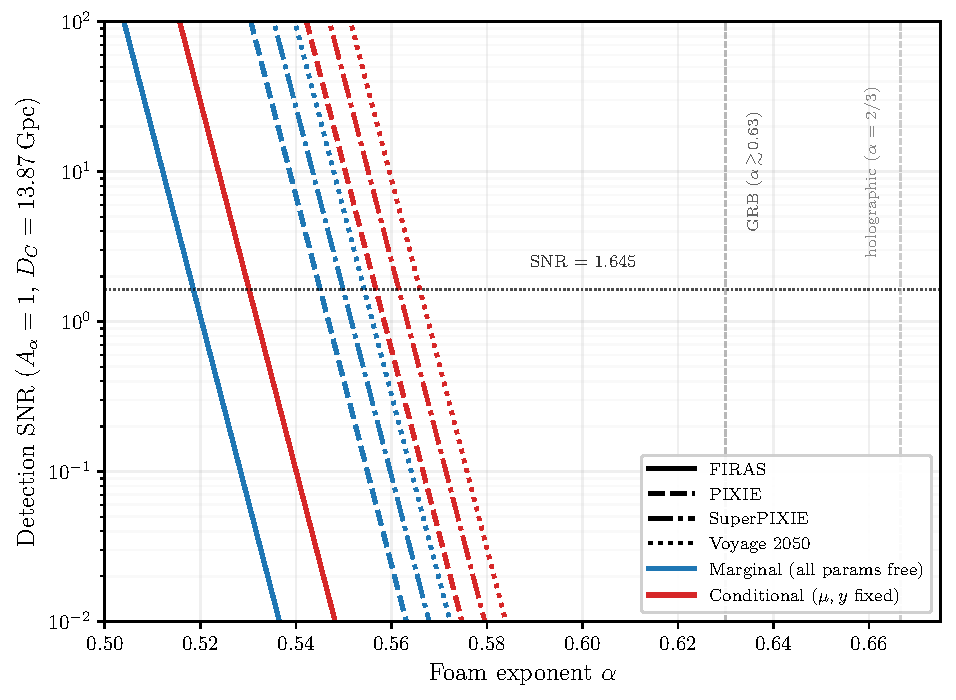
\includegraphics[width=0.82\columnwidth]{cmb_snr_alpha}
\caption{Detection SNR for the foam amplitude $A_{\rm eff}$ versus
foam exponent $\alpha$ ($A_\alpha=1$, $D_C=13.87$\,Gpc).
Blue curves: marginal SNR (all four parameters $A_{\rm eff},T_0,\mu,y$ free).
Red curves: conditional SNR ($\mu,y$ held fixed), $\sim 27\times$ higher.
Line styles denote the instrument: solid FIRAS, dashed PIXIE,
dash-dotted SuperPIXIE, dotted Voyage~2050, with forecast
$\mu$-sensitivities scaled relative to FIRAS \cite{Chluba2021}.
The marginal lower bounds cluster at $\alpha\approx 0.52$--$0.55$,
showing the logarithmic saturation of the bound with sensitivity.
The dotted horizontal line marks SNR\,$=1.645$ (one-sided $95\%$ CL); vertical dashed lines mark the
spectroscopic lower bound from GRB\,221009A ($\alpha\gtrsim 0.63$) and the
holographic prediction $\alpha=2/3$.}
\label{fig:cmb_snr}
\end{figure}

To bound the impact of $\mu$-aligned in-band pedestal contamination, we
repeat the analysis with the $\mu$-aligned band-filling kernel of
Section~\ref{sec:CMB_derivation}, replacing the deficit by
\begin{equation}
  \frac{\partial I_\nu}{\partial A_{\rm eff}}
    = -\!\left(\frac{2\pi\nu}{c}\right)^{\!2} B_\nu(T_0)
      + K_\nu^{\rm fast}(\nu)\!\int_{\nu_{\rm min}}^{\nu_{\rm max}}
        \left(\frac{2\pi\nu'}{c}\right)^{\!2} B_{\nu'}(T_0)\,d\nu',
  \label{eq:dIdA}
\end{equation}
whose $1/\nu$ pedestal we deliberately gave the Rayleigh--Jeans shape
of the $\mu$-distortion template (Eq.~\eqref{eq:Knufast}; the
Rayleigh--Jeans limit of Eq.~\eqref{eq:dIdmu} is
$\Delta I/B\to-\mu/x\propto\nu^{-1}$) so as to maximize the foam--$\mu$
overlap.  The resulting correlation matrix for
$(A_{\rm eff},\,T_0,\,\mu,\,y)$ is
\begin{equation}
\rho^{\mu\text{-align}}_{ij} = \begin{pmatrix}
  1.000 & 0.937 & \mathbf{0.976} & 0.010 \\
  0.937 & 1.000 & 0.969 & -0.212 \\
  \mathbf{0.976} & 0.969 & 1.000 & -0.127 \\
  0.010 & -0.212 & -0.127 & 1.000
\end{pmatrix}.
\label{eq:fisher_corr_matrix}
\end{equation}
Compared with the fiducial matrix
Eq.~\eqref{eq:fisher_corr_matrix_fid}, adding the in-band pedestal
rotates the foam template off the temperature axis
($\rho_{A_{\rm eff}T_0}:0.9997\to0.937$) and off the $y$ template
($\rho_{A_{\rm eff}y}:0.999\to0.010$), leaving the engineered
foam--$\mu$ degeneracy ($\rho_{A_{\rm eff}\mu}=0.976$, bold) as the
dominant one.  Since $0.976<0.9997$, the amplitude is in fact \emph{better} constrained,
\begin{equation}
  \sigma(A_{\rm eff}) = 1.7\times10^{-12}\,{\rm m}^2,
  \qquad
  \sigma(A_{\rm eff})\big|_{\mu,y\,\text{fixed}}
    = 2.9\times10^{-13}\,{\rm m}^2,
  \label{eq:sigma_Aeff_adv}
\end{equation}
a factor $\sim 6$ marginalization penalty driven by the foam--$\mu$
collinearity, and the threshold \emph{tightens} slightly to
$\alpha\gtrsim 0.53$.  The $\mu$-aligned in-band pedestal therefore does
not loosen the bound: the factor $N\approx 13$ between the
two amplitude uncertainties is compressed by the logarithmic Ng--Perlman
relation $\sigma_\ell^2 = D_C^{2(1-\alpha)}\ell_P^{2\alpha}$ into a
negligible shift $\Delta\alpha=\ln N/[2\ln(D_C/\ell_P)]\approx 0.009$.
An external constraint on $\mu$ helps most in this $\mu$-limited regime: imposing the $\Lambda$CDM dissipation prediction
$\mu\approx 2\times10^{-8}$~\cite{Chluba2021} as a prior (five orders
of magnitude tighter than the FIRAS $\mu$ measurement, hence
effectively fixing $\mu$) sharpens $\sigma(A_{\rm eff})$ by
$\sim 3$--$5\times$, though the logarithmic relation again limits the
threshold gain to $\Delta\alpha\lesssim 0.005$; in the physical
no-pedestal case, where the limiting degeneracy is with $T_0$ rather
than $\mu$, even fixing $\mu$ barely helps.  Either way, the worked
example of Section~\ref{sec:CMB_derivation} shows that any
exponential-class $C_\alpha$ with Planck-scale $\tau_{\rm foam}$ lies
in the no-pedestal regime, so the physical $\alpha\gtrsim 0.52$ is the
headline and the $\mu$-aligned $\alpha\gtrsim 0.53$ merely confirms its
robustness.

The proposed PIXIE satellite~\cite{Kogut2011} --- a fully cryogenic
($T_{\rm sys}\approx2.7$\,K) nulling polarizing Fourier transform spectrometer
spanning $30$\,GHz to $6$\,THz --- is projected to surpass FIRAS sensitivity
by roughly three orders of magnitude, reaching $|\mu|\lesssim10^{-8}$ and
$|y|\lesssim10^{-9}$ and entering the regime of guaranteed $\Lambda$CDM
spectral signals from Silk damping and reionization.
Propagating this gain through the Fisher-matrix scaling derived above,
the marginal foam detection threshold shifts from
$\alpha\gtrsim0.52$ (FIRAS) to approximately $\alpha\gtrsim0.54$
(PIXIE; Table~\ref{tab:thresholds}), narrowing the gap with the
spectroscopic lower bound $\alpha\gtrsim0.63$ from GRB\,221009A
(Fig.~\ref{fig:cmb_snr}).  All thresholds are quoted for the physical
no-pedestal deficit.  The step sizes track the logarithm of the
sensitivity ratio --- each decade of $\sigma(\mu)$ buys only
$\Delta\alpha=\ln10/[2\ln(D_C/\ell_P)]\approx0.008$ --- so the
$\sim\!3$-decade FIRAS$\to$PIXIE gain accounts for the $\approx0.03$
step, whereas PIXIE$\to$Voyage~2050 (under a decade combined) adds only
$\approx0.009$; the thresholds saturate monotonically (the three forecast
entries round $0.545$, $0.549$, $0.554$ to $0.54$--$0.55$).
The limiting degeneracy --- with a temperature shift for the
no-pedestal deficit --- persists on the linearized template.  But
PIXIE's extension to $6$\,THz accesses the nonlinear regime
$\sigma_\phi^2\gg1$ for $\alpha\lesssim0.52$ (higher $\alpha$ than
the FIRAS-band crossing $\alpha\lesssim0.50$,
Section~\ref{sec:CMB_degeneracy}, because the wider $6$\,THz band pushes
the $\sigma_\phi^2=1$ boundary upward), where the foam deficit
diverges markedly from the blackbody and $\mu$-distortion shapes
and the degeneracy may be substantially reduced.  The
$\alpha\gtrsim0.54$ projection may therefore understate the reach: if
the nonlinear template effectively breaks this degeneracy at PIXIE
sensitivity, the true threshold could be significantly more stringent.

Extending the same Fisher analysis to the $10$\,GHz--$3$\,THz bands of
the SuperPIXIE and Voyage~2050 concepts~\cite{Chluba2021} --- with
forecast distortion sensitivities
$\sigma(\mu)\approx 7.7\times10^{-9}$ and $2.2\times10^{-9}$ ---
shifts the marginal threshold only to $\alpha\gtrsim 0.55$
(Table~\ref{tab:thresholds}), barely beyond the
PIXIE projection.  The reason is structural rather than instrumental:
in the no-pedestal limit the foam deficit
$-\sigma_\phi^2(\nu)B_\nu$ is degenerate with a temperature shift at
$\rho^{\rm fid}_{A_{\rm eff}T_0}=0.9997$, and this degeneracy is
\emph{band-robust} --- broadening coverage from the FIRAS band to
$10$\,GHz--$6$\,THz leaves it unchanged to four decimal places.  The
wider band does break the foam--$\mu$ degeneracy probed by the
$\mu$-aligned $K_\nu^{\rm fast}$ pedestal (from
$\rho^{\mu\text{-align}}_{A_{\rm eff}\mu}=0.98$ at FIRAS to $0.66$ over
$10$\,GHz--$3$\,THz), so future missions are markedly more robust
against in-band pedestal contamination, but the physical threshold does
not move.  With the logarithmic Ng--Perlman scaling
$\Delta\alpha=\ln N/[2\ln(D_C/\ell_P)]$ converting even a
$10^{4}$-fold sensitivity gain over FIRAS into
$\Delta\alpha\lesssim 0.04$, this sets a firm ceiling: as an
independent broadband probe --- absolute calibrated photometry, no
source-profile assumption, a different systematic-error budget from
spectroscopy --- spectral-distortion photometry yields a lower bound
($\alpha\gtrsim 0.52$ from FIRAS, at most $\alpha\gtrsim 0.55$
next-generation) that cannot, by sensitivity or bandwidth alone, match
the stronger GRB bound $\alpha\gtrsim 0.63$ or reach the holographic
$\alpha=2/3$.  The two channels therefore
probe the same exponent through different sources, observables, and
systematics --- an independent cross-check rather than a joint bracket
--- with the GRB the more constraining of the two.

% ==============================================================
% CLAUDE:END-PROTECT
%xCLAUDE:PROTECT
\section{Conclusions}
\label{sec:conclusions}

Spacetime foam imprints an achromatic, stochastic arrival-time jitter
that modifies the first-order temporal coherence $g^{(1)}(\tau)$, and
hence the observed spectrum, providing a spectroscopic probe
complementary to the imaging (PSF, Strehl) channel.  In the
dynamical-foam limit the spectrum splits into a coherent line core
suppressed by $e^{-\sigma_\phi^2}$ and an incoherent pedestal, yielding
a shape-distortion bound on the Ng--Perlman exponent $\alpha$.  The MeV
emission lines of GRB\,221009A give $\alpha\gtrsim 0.63$ (one-sided
$95\%$ CL), while a fit to the COBE/FIRAS monopole gives
$\alpha\gtrsim 0.52$ ($95\%$ CL); next-generation
spectrometers (PIXIE, SuperPIXIE, Voyage~2050) reach
$\alpha\gtrsim 0.54$--$0.55$, the bound saturating logarithmically
because the foam deficit is nearly degenerate with a temperature shift.
The pedestal-independent line-width and CMB bounds do not exclude the
holographic value $\alpha=2/3$; however, the TeV survival bound
($\alpha_{\rm TeV}\gtrsim0.74$, conditional on the eikonal pedestal
kernel) would exclude it.

All single-source spectroscopic bounds derived in this paper assume the
dynamical-foam limit $\tau_{\rm foam}\ll\tau_c$
(Section~\ref{sec:closedforms}), in which the foam path-length jitter
decorrelates many times within each photon coherence time.  If foam
fluctuations are instead slow ($\tau_{\rm foam}\gg\tau_c$), the
accumulated phase is essentially frozen during each coherence time and
the foam acts as a deterministic, frequency-independent phase screen
--- no spectral broadening or peak reduction occurs within a single
observation, and the shape-distortion bounds do not apply.  The CMB
constraint (Section~\ref{sec:CMB}) is similarly derived in the
dynamical limit (Section~\ref{sec:CMB_derivation} works in
$C_\alpha\to 0$): in the opposite quasi-static limit the per-mode
foam suppression $\mathcal{F}_{\rm foam}(\tau)\to 1$
(Eq.~\eqref{eq:Ffoam}) and the CMB monopole is unmodified, so the
shape-distortion bounds do not apply in either channel.

The pedestal-independent dynamical bound $\alpha\gtrsim 0.63$
(Eq.~\eqref{eq:alpha_grb_dyn}) --- a weak, lever-arm-dominated floor ---
does not exclude the holographic value
$\alpha=2/3\approx 0.667$, though the TeV bound
(Eq.~\eqref{eq:alpha_grb_tev}, conditional on Assumption~(ii))
would.  A principal instrumental limitation of the
present analysis is the MeV sensitivity gap: the spectral region
between the upper edge of the Fermi-GBM BGO detector response
($\lesssim40\,\mathrm{MeV}$, where the effective area falls steeply)
and the regime in which Fermi-LAT achieves robust detection efficiency
($\gtrsim100\,\mathrm{MeV}$).
The frequency $\nu_\star \simeq 37\,\mathrm{MeV}$ at which the foam-induced
spectral break is predicted to be most constraining falls squarely within
this gap, so neither instrument provides fully resolved coverage across
the critical transition.
Closing the MeV gap is a recognized community priority, addressed by
next-generation satellite concepts that combine Compton-scattering and
pair-conversion detection techniques to achieve continuous sensitivity from
$\sim100\,\mathrm{keV}$ to beyond $1\,\mathrm{GeV}$.
The All-sky Medium Energy Gamma-ray Observatory
(AMEGO~\cite{McEnery2019}) and its MIDEX-scale variant
AMEGO-X~\cite{Caputo2022} are designed to cover $100\,\mathrm{keV}$ to
$1\,\mathrm{GeV}$ with order-of-magnitude improvements over both COMPTEL
and Fermi-LAT in the MeV decade; the ESA-proposed M-class concept
e-ASTROGAM~\cite{DeAngelis2017} targets a comparable bandpass.
The near-term NASA SMEX mission COSI (scheduled launch $\sim$2027)
will extend broadband sensitivity to $0.2$--$5\,\mathrm{MeV}$, providing
a valuable pathfinder, though its upper energy bound falls well short of
the $37\,\mathrm{MeV}$ regime and the gap therefore remains open.
Realization of any of the broader-bandpass concepts would, for the first
time, permit fully resolved spectral measurements of GRB prompt emission
across the $37\,\mathrm{MeV}$ transition without the instrumental
discontinuity that limits the present work; reducing the per-epoch
line-width uncertainties to $\delta r\lesssim 0.01$ would tighten the
bound to $\alpha\gtrsim 0.64$, removing a major systematic and
enabling substantially tighter tests of spacetime-foam models.
Independently, a joint fit of the line centroid and width across epochs
--- the present analysis constrains the width alone --- would exploit
the energy-dependent line-center shift
$\nu_0^{\rm eff}=\nu_0\,\tau_G^2/(\tau_G^2+\sigma_\Delta^2)$
(Eq.~\eqref{eq:Sobs_gauss}) that the same foam jitter induces, adding a
second handle on $\alpha$ and further tightening the bound.

A complementary implication runs in the opposite direction.  The
flagship goal of next-generation CMB spectrometers --- PIXIE,
SuperPIXIE, Voyage~2050 --- is a first detection of the chemical
potential $\mu$, whose guaranteed $\Lambda$CDM value
$\mu\simeq2\times10^{-8}$ arises from Silk damping of primordial
perturbations.  Our Fisher analysis shows that the foam-induced
distortion is nearly degenerate with the $\mu$ template across the
accessible band (Section~\ref{sec:CMB_degeneracy}); the two cannot be
separated from the monopole spectrum alone.  A measured $\mu$ that
\emph{departs} from the $\Lambda$CDM prediction would be a landmark
signal whatever its origin, and spacetime foam is one
propagation-induced alternative to early-universe energy injection ---
distinguishable only with external information.  The GRB lower bound
$\alpha\gtrsim0.63$ already limits any foam contribution to the CMB
monopole to far below the $\Lambda$CDM $\mu$, so foam does not
contaminate the guaranteed-$\mu$ target; but this same
spectroscopy-plus-GRB complementarity is what would be needed to
attribute a larger, anomalous $\mu$.  In this sense the CMB
$\mu$-distortion measurement and the foam search are two readings of a
single spectral degeneracy.  The decisive limitation here is
theoretical rather than instrumental: the pedestal shape --- and hence
how completely the foam deficit can be separated from a temperature
shift or from $\mu$ --- is fixed by the foam temporal autocorrelation
$C_\alpha(\tau)$, which still awaits a first-principles derivation from
a quantum-gravity model. The amplitude $A$ itself is in the same position:
it is calibrated phenomenologically rather than derived from a
fluctuation-dissipation or holographic-entropy argument at the Planck-cell
level.

The multi-epoch $r_{\rm obs}$ dataset constrains any propagation
effect that broadens an emission line in proportion to a power of
$E$, not only the Ng--Perlman spacetime-foam template considered
here.  The most natural extension is to stochastic Lorentz-invariance
violation~\cite{AmelinoCamelia2013}, in which the photon group
velocity carries a Planck-suppressed random coefficient
$v(E)=c\bigl[1-\xi\,(E/E_{\rm QG,n})^n\bigr]$, with $\xi$ of order
unity drawn independently for each Planck-scale traversal.  Photons
in the same line then propagate at slightly different speeds,
broadening the observed width as
$\sigma_{\rm LIV}(E)/E\propto E^n$ on top of any intrinsic
contribution.  Unlike the deterministic LIV signal probed by photon
time-of-flight studies~\cite{Fermi2009} --- where GRB\,221009A LHAASO TeV photons
already constrain $E_{\rm QG,1}\gtrsim$ a
few~$\times\,E_{\rm Pl}$~\cite{LHAASOTeV2023} --- stochastic LIV
produces a \emph{width} signal that survives light-curve
cross-correlation, and a multi-epoch $r_{\rm obs}$ measurement is
therefore one of the few clean probes available.  Fitting
Eq.~\eqref{eq:robs_model} recovers the foam constraint as the
$n=1$ case; refitting the same seven-epoch dataset under
$r_{\rm LIV}\propto(E/E_0)^n$ would yield bounds on
$\langle\xi^2\rangle^{1/2}/E_{\rm QG,n}^n$ at each order, with the
$n=2$ (quadratic) case particularly valuable because the
deterministic time-of-flight tests are weakest there at $z=0.151$.

\begin{acknowledgments}
This work was supported in part by the Director, Office of Science, Office of
High Energy Physics of the U.S.\ Department of Energy under Contract No.\
DE-AC02-05CH11231.

The authors used Claude (Anthropic) and Valency Systems to assist with drafting and editing portions of this manuscript, with detailed reference searches, and in developing the Fisher-matrix and GRB multi-epoch analysis scripts. All content, equations, numerical results, and conclusions were reviewed and verified by the authors, who take full responsibility for the work.  AI assistance was used in accordance with \textit{Physical Review} editorial policy on computational tools.

We thank Robin Kaiser for helpful discussions that helped motivate this work, and Eric Linder for an insightful comments.
\end{acknowledgments}

\bibliographystyle{apsrev4-2}
\bibliography{../references}
% CLAUDE:END-PROTECT
\end{document}
